% Chapter generated from d7948fc8-horseshoe_ftns.tex
% chapter macros
\chapter{The Horseshoe and the Fundamental Theorem of Natural Selection}\label{ch:hs}
\chaptermark{The Horseshoe and the Fundamental Theorem}
\begin{chaptersummary}
Ewens's reading of Fisher's Fundamental Theorem identifies the partial change in mean fitness with the additive genetic variance in fitness divided by mean fitness. Once the average effects are recognized as the coefficients of a weighted least squares regression of genotypic fitness on allelic dosage, the theorem is a one line algebraic identity and the whole of its empirical content is transferred to the estimation of a regression. That regression is overparameterized: there are more loci than individuals, the ordinary estimator of the additive variance is inflated by $L\sigma^2_\varepsilon/n$, and the implied rate of adaptation is correspondingly overstated. I propose estimating the average effects under a horseshoe prior and reading the Fundamental Theorem through the resulting shrinkage weights, which yields a rate of adaptation discounted by a signal to noise factor that is estimated rather than assumed. Three results are given: any shrinkage rule delivers a conservative estimate of the rate; oracle shrinkage tuned for the average effects necessarily understates the additive variance; and the coherent estimator is the posterior mean of the quadratic functional, not the quadratic of the posterior mean. In simulation with $L = 400$ loci and $n = 300$ individuals the naive estimator overstates the additive variance by a factor of $3.2$, ridge returns only $0.40$ of it, and the horseshoe posterior recovers it to within $8\%$. Four further questions are then taken up. Posterior intervals for the quadratic functional cover at $85\%$ against a nominal $90\%$, and in $600$ replicates $80$ of the $91$ misses lie above the truth; the regularized horseshoe covers at $89\%$, close to the nominal level. Robertson's secondary theorem requires a bilinear functional whose plug in carries a bias $L\rho\sigma_w\sigma_z/n$ in the residual correlation; a bivariate horseshoe with shared local scales reduces a $2.6$ fold overstatement to a $17\%$ understatement. Under linkage disequilibrium the estimand is $\alpha^\top V\alpha$ rather than a diagonal form, and a shrinkage plug in that keeps the diagonal form loses a further nine percent of the truth, although in the design simulated the posterior mean is nearly insensitive to the choice. Ascertainment is not a shrinkage problem at all: measuring fitness on survivors understates the additive variance almost fourfold, and no prior repairs it. The choice between a horseshoe and a Gaussian prior encodes the sweep versus infinitesimal question about genetic architecture, and the Fundamental Theorem inherits the answer.
\end{chaptersummary}
\section{Introduction}

Fisher's Fundamental Theorem of Natural Selection asserts that the rate of increase in fitness of any organism at any time is equal to its genetic variance in fitness at that time \citep{hs:fisher1930genetical}. For four decades the statement was read as a claim about the total change in mean fitness, in which form it is simply false, and it acquired a reputation for obscurity that it did not deserve. The modern understanding is due principally to \citet{hs:price1972fisher} and to \citet{hs:ewens1989interpretation}: the theorem concerns the \emph{partial} change in mean fitness, the part ascribable to changes in allele frequency with the average effects held at their current values, and in that reading it is exact. \citet{hs:ewens2004mathematical} and \citet{hs:ewens2015interpretation} give the definitive treatment; \citet{hs:edwards1994fundamental} and \citet{hs:lessard1997fisher} supply complementary accounts.


The history is worth a paragraph, because the shape of the confusion explains the shape of what remains. Fisher stated the theorem in one sentence in 1930 and gave a derivation that almost no one followed. \citet{hs:price1972fisher} reconstructed the argument and showed that Fisher had been careful and had been read carelessly: the theorem concerns a partial derivative, and the counterexamples in the literature were all constructed by varying quantities Fisher had explicitly held constant. \citet{hs:ewens1989interpretation} supplied the modern proof and, crucially, the account of \emph{why} the partial change is the object of interest rather than a mathematical convenience; \citet{hs:ewens2015interpretation} assess how much biological work the theorem does once correctly stated, and conclude, in my reading, that it does less than Fisher hoped but more than his critics allowed. That literature is settled. What follows takes it as given and asks only what happens when one tries to use it on data.

This chapter takes a statistician's view of what remains after the interpretive question is settled. The central observation is that Fisher's average effect of an allele is, by construction, a coefficient in a weighted least squares regression of genotypic fitness on allelic dosage, and the additive genetic variance is the regression sum of squares from that fit. The Fundamental Theorem is then an algebraic identity relating a regression sum of squares to a one generation increment, and it is true whatever the data. All of its empirical content sits in the estimation of the regression.

That regression, in any modern application, is severely overparameterized. Fitness or a fitness proxy is measured on $n$ individuals genotyped at $L \gg n$ loci. The ordinary least squares or marginal estimator of the average effects overfits, the plug in estimator of the additive variance inherits an upward bias of order $L\sigma^2_\varepsilon/n$, and the rate of adaptation implied by the Fundamental Theorem is inflated by the same amount. The theorem is not at fault. The estimator is.

\paragraph{Plan of the chapter.} I propose estimating the average effects under a horseshoe prior \citep{hs:carvalho2010horseshoe,hs:polson2012local} and reading the Fundamental Theorem through the induced shrinkage weights. Section~\ref{hs:sec:ftns} sets out the theorem as a least squares identity (Proposition~\ref{hs:prop:ftns}) and isolates the remainder term. Section~\ref{hs:sec:bias} gives the bias of the plug in estimator in closed form (Proposition~\ref{hs:prop:bias}). Section~\ref{hs:sec:hs} develops the horseshoe version: any shrinkage rule yields a conservative rate (Proposition~\ref{hs:prop:conservative}); oracle shrinkage tuned for estimating the average effects necessarily understates the additive variance (Proposition~\ref{hs:prop:oracle}); and the coherent Bayesian estimator is the posterior mean of the quadratic functional, which restores what the plug in loses (Proposition~\ref{hs:prop:posterior}). Section~\ref{hs:sec:sim} reports a simulation. Section~\ref{hs:sec:secondary} extends the argument to Robertson's secondary theorem and to Lande Arnold selection gradients, where the same pathology is if anything worse. Section~\ref{hs:sec:open} takes up four problems the propositions leave open: calibration, the bilinear functional, linkage disequilibrium and ascertainment. Throughout, small worked examples with numbers a reader can check by hand accompany the general results: a single locus with dominance, a stylized overdominant polymorphism, a regression with five loci and eight individuals, a table of horseshoe shrinkage weights, and an exact calculation of the damage done by truncation selection. The chapter closes with exercises.

\paragraph{A remark on what is being claimed.} Nothing here revises the Fundamental Theorem, and nothing here is a criticism of it. The claim is that the theorem, correctly understood, converts a question about evolution into a question about a high dimensional regression, and that the statistical literature has an answer to the second question which the evolutionary literature has not generally adopted.

\section{The theorem as a least squares identity}
\label{hs:sec:ftns}

\subsection{Setup}

Consider a single locus with alleles $A_1,\ldots,A_k$ at frequencies $p = (p_1,\ldots,p_k)$, random mating, and constant genotypic fitnesses $w_{ij} = w_{ji}$. The mean fitness and the marginal fitness of $A_i$ are
\[
\bar w = \sum_{i,j} p_i p_j w_{ij}, \qquad w_i = \sum_j p_j w_{ij},
\]
and the standard viability selection recursion is $p_i' = p_i w_i/\bar w$, so that
\begin{equation}
\Delta p_i = \frac{p_i (w_i - \bar w)}{\bar w}.
\label{hs:eq:recursion}
\end{equation}

Fisher's average effect $\alpha_i$ is defined as the solution of a weighted least squares problem: the additive model $w_{ij} \approx \mu + \alpha_i + \alpha_j$ is fitted by minimizing
\begin{equation}
Q(\alpha) = \sum_{i,j} p_i p_j \big(w_{ij} - \mu - \alpha_i - \alpha_j\big)^2
\label{hs:eq:wls}
\end{equation}
subject to $\sum_i p_i \alpha_i = 0$. The weights are the genotype frequencies under random mating, $p_ip_j$ for the ordered genotype $(i,j)$. The next subsection shows that the solution is $\mu = \bar w$ and $\alpha_i = w_i - \bar w$. The additive genetic variance in fitness is the explained sum of squares,
\[
\sigma^2_A = \sum_{i,j} p_ip_j(\alpha_i+\alpha_j)^2 = 2\sum_i p_i \alpha_i^2 = 2\sum_i p_i (w_i - \bar w)^2,
\]
where the cross term $2\sum_{i,j}p_ip_j\alpha_i\alpha_j = 2(\sum_i p_i\alpha_i)^2$ vanishes by the constraint, and the dominance variance $\sigma^2_D = Q(\alpha)$ is the residual sum of squares in \eqref{hs:eq:wls} at the minimum. This is the whole of the construction: average effects are regression coefficients, additive variance is a regression sum of squares, dominance variance is a residual. \citet{hs:ewens2004mathematical} is emphatic on this point, and it is the point on which everything below turns.


\subsection{The normal equations}

Since everything below rests on the regression interpretation, it is worth writing the normal equations out in full. Write $r_{ij} = w_{ij} - \mu - \alpha_i - \alpha_j$ for the residual of genotype $(i,j)$; note $r_{ij} = r_{ji}$. The parameter $\alpha_i$ enters $Q$ through every residual $r_{ij}$ and every residual $r_{ji}$, so
\[
\frac{\partial Q}{\partial \alpha_i} = -2\sum_j p_ip_j r_{ij} - 2\sum_j p_jp_i r_{ji} = -4p_i\sum_j p_j r_{ij},
\qquad
\frac{\partial Q}{\partial \mu} = -2\sum_{i,j}p_ip_jr_{ij}.
\]
Minimize $Q$ first without the constraint. Setting the $\mu$ derivative to zero and using $\sum_{i,j}p_ip_jw_{ij} = \bar w$ gives
\[
\bar w - \mu - 2\textstyle\sum_j p_j\alpha_j = 0 .
\]
Setting the $\alpha_i$ derivative to zero (and dividing by $4p_i > 0$) gives, for each $i$,
\[
\sum_j p_j \big(w_{ij} - \mu - \alpha_i - \alpha_j\big) = 0
\quad\Longrightarrow\quad
w_i - \mu - \alpha_i - \textstyle\sum_j p_j\alpha_j = 0 .
\]
These $k+1$ equations have one degree of freedom too many: adding a constant $c$ to every $\alpha_i$ and subtracting $2c$ from $\mu$ leaves every fitted value unchanged. The constraint $\sum_j p_j \alpha_j = 0$ removes that freedom, and then the first equation gives $\mu = \bar w$ and the second gives $\alpha_i = w_i - \bar w$. As a check, this solution does satisfy the constraint, since $\sum_i p_i w_i = \bar w$. The constraint is therefore an identification convention and not a restriction: the fitted values $\mu + \alpha_i + \alpha_j$, and hence $\sigma^2_A$ and $\sigma^2_D$, are the same under any convention. The simplification is a consequence of random mating, which makes the design matrix of the regression orthogonal in the appropriate weighted inner product. Under nonrandom mating the normal equations do not decouple and $\alpha$ must be obtained by solving a genuine weighted least squares system, in which case $\alpha_i \ne w_i - \bar w$ but Proposition~\ref{hs:prop:ftns} continues to hold with $\sigma^2_A$ redefined as the explained sum of squares of that system. This is the generality emphasized by \citet{hs:ewens2004mathematical}: the theorem is a property of the projection, not of the particular mating scheme that makes the projection easy to compute.

\subsection{The identity}

\begin{proposition}[Fundamental Theorem]
\label{hs:prop:ftns}
Define the partial change in mean fitness as the change generated by the frequency increments \eqref{hs:eq:recursion} with the average effects held fixed,
\[
\Delta_\alpha \bar w := 2\sum_i \alpha_i \,\Delta p_i .
\]
Then $\Delta_\alpha \bar w = \sigma^2_A/\bar w$.
\end{proposition}

\begin{proof}
Substituting $\alpha_i = w_i - \bar w$ and \eqref{hs:eq:recursion},
\[
2\sum_i \alpha_i \Delta p_i
= 2\sum_i (w_i - \bar w)\,\frac{p_i(w_i-\bar w)}{\bar w}
= \frac{2}{\bar w}\sum_i p_i (w_i - \bar w)^2
= \frac{\sigma^2_A}{\bar w}. \qedhere
\]
\end{proof}

The proof is three lines because the theorem is an identity. It says that if one defines the average effects by least squares and then asks how much of the change in mean fitness is attributable to frequency change through those effects, the answer is the explained sum of squares divided by $\bar w$. The content is in the definition, not the derivation, which is precisely why the theorem was misunderstood for so long: read as a claim about $\Delta \bar w$ it is false, and read as a claim about $\Delta_\alpha \bar w$ it is trivial. What makes it substantive is that $\Delta_\alpha \bar w$ is the evolutionarily meaningful component, the part driven by selection acting on heritable variation, as opposed to the part driven by the environment changing underfoot \citep{hs:ewens1989interpretation,hs:ewens2015interpretation}.

\begin{example}[One locus with partial dominance]
\label{hs:ex:onelocus}
Take two alleles with $p_1 = 0.2$, $p_2 = 0.8$ and genotypic fitnesses $w_{11} = 1.10$, $w_{12} = 1.06$, $w_{22} = 1.00$. In the usual parameterization the homozygote midpoint is $1.05$, the additive effect is $a = 0.05$ and the dominance deviation is $d = 0.01$. The marginal fitnesses are
\[
w_1 = 0.2(1.10) + 0.8(1.06) = 1.068, \qquad w_2 = 0.2(1.06) + 0.8(1.00) = 1.012,
\]
and $\bar w = p_1w_1 + p_2w_2 = 0.2136 + 0.8096 = 1.0232$. The average effects are $\alpha_1 = 0.0448$ and $\alpha_2 = -0.0112$; their weighted sum $0.2(0.0448) + 0.8(-0.0112)$ is zero, as it must be. The average effect of substituting allele 1 for allele 2 is $\alpha_1 - \alpha_2 = 0.056$, which agrees with $a + d(1-2p_1) = 0.05 + 0.01(0.6)$. Then
\[
\sigma^2_A = 2\big[0.2(0.0448)^2 + 0.8(0.0112)^2\big] = 0.00100352,
\]
which equals $h(\alpha_1-\alpha_2)^2$ with $h = 2p_1p_2 = 0.32$, and the dominance variance is $\sigma^2_D = (hd)^2 = (0.0032)^2 = 1.024\times10^{-5}$. Dominance contributes one percent of the genetic variance in fitness. The recursion gives $\Delta p_1 = 0.2(0.0448)/1.0232 = 0.0087568$, so Fisher's partial change is
\[
\Delta_\alpha \bar w = 2\big[\alpha_1\Delta p_1 + \alpha_2\Delta p_2\big] = 2(0.056)(0.0087568) = 0.00098077 = \sigma^2_A/\bar w ,
\]
using $\Delta p_2 = -\Delta p_1$. Evaluating $\bar w$ directly at $p_1' = 0.2087568$ gives a total change of $0.00097923$. The remainder is $R = -1.5\times10^{-6}$; since $\bar w$ is a quadratic in $p_1$ with second difference $w_{11} - 2w_{12} + w_{22} = -2d$, it is exactly $R = -2d(\Delta p_1)^2 = -0.02(0.0087568)^2$ (Exercise~\ref{hs:exr:remainder}). The realized change is $99.84\%$ of the partial change. With selection coefficients of five percent and one locus, Fisher's term is almost the whole story.
\end{example}

\subsection{The remainder}

The total change decomposes as
\begin{equation}
\Delta \bar w = \underbrace{\frac{\sigma^2_A}{\bar w}}_{\text{partial change}} + \ R,
\label{hs:eq:decomp}
\end{equation}
where $R$ collects the change in mean fitness due to the average effects themselves shifting as frequencies change, together with any change in the genotypic fitnesses. For a single locus with constant $w_{ij}$ and weak selection, $R = O(\|\Delta p\|^2)$: the average effect $\alpha_i$ is a smooth function of $p$, so reevaluating it after one generation contributes at second order. With multiple loci, epistasis, frequency dependence or a changing environment, $R$ need not be small and can be negative, which is the source of every apparent counterexample to the theorem in the older literature \citep{hs:frank1992fishers}.

A numerical remark anticipating Section~\ref{hs:sec:sim}: in the simulations reported there, with $400$ loci, additive and dominance effects and weak selection, the realized $\Delta\bar w$ exceeds the partial change by a factor of $1.0004$. The remainder is negligible. The discrepancy between the theorem and reality in that setting is four hundredths of one percent, while the discrepancy introduced by estimating $\sigma^2_A$ badly is a factor of three. This ordering is the motivation for the rest of the chapter.

\begin{example}[A stylized overdominant polymorphism]
\label{hs:ex:overdominance}
The remainder can matter, and the additive variance can vanish while the genetic variance does not. Take alleles $A$ and $S$ with stylized fitnesses $w_{AA} = 0.9$, $w_{AS} = 1.0$, $w_{SS} = 0.2$, of the heterozygote advantage type usually used to illustrate the sickle cell polymorphism in malarial regions; the values are illustrative, not estimates. With selection coefficients $s = 0.1$ against $AA$ and $t = 0.8$ against $SS$, the stable equilibrium frequency of $S$ is $q^* = s/(s+t) = 1/9 \approx 0.111$.

At $q = 0.05$ one finds $\bar w = 0.90775$, average effects $\alpha_A = -0.00275$ and $\alpha_S = 0.05225$, and
\[
\sigma^2_A = 2.874\times10^{-4}, \qquad \sigma^2_D = 1.828\times10^{-3}.
\]
The dominance variance is more than six times the additive variance, so substituting the total genetic variance for the additive variance would overstate the rate more than sevenfold. Fisher's partial change is $\sigma^2_A/\bar w = 3.166\times10^{-4}$; the exact change in mean fitness, computed from the recursion, is $3.091\times10^{-4}$, so the remainder is now $2.4\%$ of the total rather than the $0.16\%$ of Example~\ref{hs:ex:onelocus}. At $q = q^*$ the marginal fitnesses are equal, $\alpha_A = \alpha_S = 0$, $\sigma^2_A = 0$ and the partial change is zero, while $\sigma^2_D = 0.0079$ remains large. At a balanced polymorphism there is abundant genetic variance in fitness and no additive variance, and the theorem correctly says that mean fitness has stopped rising.
\end{example}

\subsection{The Price equation and what the theorem is a special case of}

It is worth locating Proposition~\ref{hs:prop:ftns} within the more general covariance formalism, because doing so makes clear which part is definitional and which is substantive. The Price equation \citep{hs:price1970selection} states that for any character $z$ with values $z_i$ in the parent generation and mean $\bar z$,
\[
\bar w \, \Delta\bar z = \mathrm{Cov}(w_i, z_i) + \mathbb{E}\big[w_i\,\delta_i\big],
\]
where $\delta_i$ is the within lineage change in $z$ between parent and offspring. Setting $z = w$ gives $\bar w\,\Delta\bar w = \mathrm{Var}(w) + \mathbb{E}[w\delta]$: the change in mean fitness is the variance in fitness plus a transmission term. This is not the Fundamental Theorem, and the difference is instructive. The Price form uses the \emph{total} variance in fitness, which includes dominance and environmental components that are not transmitted; the Fundamental Theorem uses only the \emph{additive} part, which is precisely the part that survives the projection \eqref{hs:eq:wls}. The transmission term absorbs the difference. Fisher's contribution was to identify the right projection, not to write down a covariance identity, and this is why \citet{hs:price1972fisher} (who is often read as having replaced Fisher's theorem) described himself as making it clear rather than correcting it.

\subsection{The multilocus regression}

For $L$ biallelic loci in linkage equilibrium, write $g_{i\ell} \in \{0,1,2\}$ for the dosage of the focal allele in individual $i$ at locus $\ell$, with frequency $p_\ell$ and $h_\ell = 2p_\ell(1-p_\ell)$. The average effect of an allelic substitution at locus $\ell$ is $\alpha_\ell = a_\ell + d_\ell(1-2p_\ell)$ in the usual additive plus dominance parameterization, and
\begin{equation}
\sigma^2_A = \sum_{\ell=1}^{L} h_\ell\,\alpha_\ell^2 .
\label{hs:eq:s2A}
\end{equation}
The $\alpha_\ell$ are the population regression coefficients of fitness on centred dosage; equivalently, they solve
\[
\alpha = \arg\min_{b}\ \mathbb{E}\Big[\big(w - \textstyle\sum_\ell b_\ell(g_\ell - 2p_\ell)\big)^2\Big].
\]
So the estimation problem is a linear regression of measured fitness on $L$ centred genotype columns, and \eqref{hs:eq:s2A} is a weighted quadratic functional of its coefficients. Everything that is known about high dimensional regression applies verbatim.

\section{The plug in estimator and its bias}
\label{hs:sec:bias}

This section computes, exactly, how far the natural estimator of the additive variance is from its target, first for an idealized orthogonal design and then for an arbitrary one, and closes with a worked example small enough to check by hand.

Let $X \in \mathbb{R}^{n\times L}$ hold centred dosages, with columns $x_1,\ldots,x_L$, let $y$ be the measured fitness of $n$ individuals, and suppose $y = X\alpha + \varepsilon$ where the errors $\varepsilon_1,\ldots,\varepsilon_n$ are uncorrelated with mean zero and variance $\sigma^2_\varepsilon$. The residual $\varepsilon$ collects environmental noise, measurement error and the dominance and epistatic deviations, which are uncorrelated with additive dosage by construction of the projection. The estimator in universal use is the plug in: estimate each $\alpha_\ell$, square, and weight by $h_\ell$ according to \eqref{hs:eq:s2A}.

\begin{proposition}[Bias of the plug in]
\label{hs:prop:bias}
Suppose the columns of $X$ are orthogonal, $x_\ell^\top x_m = 0$ for $\ell \ne m$, with $x_\ell^\top x_\ell = n h_\ell$, and let $\hat\alpha^{\rm marg}_\ell = x_\ell^\top y/(x_\ell^\top x_\ell)$. Then
\begin{enumerate}[label=(\alph*)]
\item $\displaystyle\mathbb{E}\Big[\sum_\ell h_\ell (\hat\alpha^{\rm marg}_\ell)^2\Big]
= \sigma^2_A + \frac{L\,\sigma^2_\varepsilon}{n}$;
\item if in addition $\varepsilon \sim N(0,\sigma^2_\varepsilon I_n)$, then
$\displaystyle\mathrm{Var}\Big[\sum_\ell h_\ell (\hat\alpha^{\rm marg}_\ell)^2\Big]
= \frac{4\sigma^2_\varepsilon\sigma^2_A}{n} + \frac{2L\sigma^4_\varepsilon}{n^2}$.
\end{enumerate}
\end{proposition}

\begin{proof}
Substituting $y = X\alpha + \varepsilon$,
\begin{align*}
\hat\alpha^{\rm marg}_\ell = \frac{x_\ell^\top\big(\sum_m x_m\alpha_m + \varepsilon\big)}{n h_\ell}
&= \frac{n h_\ell\,\alpha_\ell}{n h_\ell} + \sum_{m\ne\ell}\frac{x_\ell^\top x_m}{nh_\ell}\alpha_m + \frac{x_\ell^\top\varepsilon}{nh_\ell}\\
&= \alpha_\ell + e_\ell,
\qquad e_\ell = \frac{x_\ell^\top\varepsilon}{nh_\ell},
\end{align*}
the middle sum vanishing by orthogonality. The error $e_\ell$ has mean zero and variance $x_\ell^\top(\sigma^2_\varepsilon I)x_\ell/(nh_\ell)^2 = \sigma^2_\varepsilon/(nh_\ell) =: v_\ell$, and $\mathrm{Cov}(e_\ell,e_m) = \sigma^2_\varepsilon x_\ell^\top x_m/(n^2h_\ell h_m) = 0$ for $\ell\ne m$. For (a),
\[
\mathbb{E}\big[h_\ell(\alpha_\ell + e_\ell)^2\big] = h_\ell\alpha_\ell^2 + 2h_\ell\alpha_\ell\,\mathbb{E}e_\ell + h_\ell\,\mathbb{E}e_\ell^2 = h_\ell\alpha_\ell^2 + h_\ell v_\ell = h_\ell\alpha_\ell^2 + \frac{\sigma^2_\varepsilon}{n},
\]
and summing over the $L$ loci gives $\sigma^2_A + L\sigma^2_\varepsilon/n$. For (b), under normality the $e_\ell$ are uncorrelated jointly Gaussian and therefore independent, so the variance of the sum is the sum of the variances. For $e \sim N(0,v)$ one has $\mathrm{Var}\big((\alpha+e)^2\big) = \mathrm{Var}(2\alpha e + e^2) = 4\alpha^2 v + 2v^2$, since $\mathrm{Cov}(e,e^2) = \mathbb{E}e^3 = 0$ and $\mathrm{Var}(e^2) = 3v^2 - v^2$. Hence
\[
\mathrm{Var}\big[h_\ell(\hat\alpha^{\rm marg}_\ell)^2\big] = h_\ell^2\big(4\alpha_\ell^2 v_\ell + 2v_\ell^2\big) = \frac{4\sigma^2_\varepsilon}{n}h_\ell\alpha_\ell^2 + \frac{2\sigma^4_\varepsilon}{n^2},
\]
and summing over $\ell$ gives (b).
\end{proof}

The bias is $L\sigma^2_\varepsilon/n$: it does not depend on the allele frequencies, it grows linearly in the number of loci, and it does not shrink when more loci are genotyped on the same individuals; it only shrinks when more individuals are measured. When $L > n$ and the true additive variance is a modest fraction of the phenotypic variance (the normal situation) the bias exceeds the quantity being estimated. Through Proposition~\ref{hs:prop:ftns}, the implied rate of adaptation is inflated by the same factor.

Part (b) says something less obvious. Subtracting the known bias does not rescue the plug in when $L$ is large: the debiased estimator $\sum_\ell h_\ell(\hat\alpha^{\rm marg}_\ell)^2 - L\sigma^2_\varepsilon/n$ is unbiased, but its standard deviation contains the term $\sqrt{2L}\,\sigma^2_\varepsilon/n$, the accumulated noise of $L$ squared errors, and this is not removed by centring. With the values of Section~\ref{hs:sec:sim}, $L = 400$, $n = 300$, $\sigma^2_\varepsilon = 0.0320$ (the phenotypic variance, which a single locus regression treats as error) and $\sigma^2_A = 0.0205$, the bias is $0.0427$, the expected plug in is $3.08$ times the truth, and the standard deviation of the debiased estimator is $0.0042$, about a fifth of the quantity being estimated; half of its variance comes from the term $2L\sigma^4_\varepsilon/n^2$, to which every locus contributes equally whether it is causal or not. The debiased estimator can also be negative.

\paragraph{Standardized units.} It is convenient to measure each average effect in units of its own sampling standard deviation. Put
\[
\theta_\ell = \frac{\alpha_\ell}{\sqrt{v_\ell}} = \frac{\alpha_\ell\sqrt{n h_\ell}}{\sigma_\varepsilon},
\qquad
z_\ell = \frac{\hat\alpha^{\rm marg}_\ell}{\sqrt{v_\ell}} \sim N(\theta_\ell, 1),
\qquad\text{so that}\qquad
\sigma^2_A = \frac{\sigma^2_\varepsilon}{n}\sum_\ell \theta_\ell^2 .
\]
In these units the additive variance is a multiple of the squared length of a normal means vector, the plug in is the same multiple of $\sum_\ell z_\ell^2$, and Proposition~\ref{hs:prop:bias}(a) is the statement $\mathbb{E}z_\ell^2 = \theta_\ell^2 + 1$. Each locus, whether causal or not, adds one unit of $\sigma^2_\varepsilon/n$ to the expected plug in. The horseshoe calculations of Section~\ref{hs:sec:hs} are carried out in these units.

\subsection{An arbitrary design}

Orthogonality is never exactly true in a sample. For a general full rank design with $L < n$ the natural estimator is ordinary least squares, $\hat\alpha = (X^\top X)^{-1}X^\top y$, and two versions of the functional are in use: the diagonal form $\sum_\ell \hat h_\ell\hat\alpha_\ell^2$ with $\hat h_\ell = x_\ell^\top x_\ell/n$, and the full form $\hat\alpha^\top\hat V\hat\alpha$ with $\hat V = X^\top X/n$, the sample covariance matrix of the dosages. The next result shows that they have different biases, and that the full form is the better behaved.

\begin{proposition}[Bias under an arbitrary design]
\label{hs:prop:biasols}
Let $X$ have full column rank and let $\mathrm{VIF}_\ell = (X^\top X)_{\ell\ell}\,\big[(X^\top X)^{-1}\big]_{\ell\ell}$ be the variance inflation factor of locus $\ell$. Then
\[
\mathbb{E}\big[\hat\alpha^\top\hat V\hat\alpha\big] = \alpha^\top\hat V\alpha + \frac{L\sigma^2_\varepsilon}{n},
\qquad
\mathbb{E}\Big[\sum_\ell \hat h_\ell\hat\alpha_\ell^2\Big] = \sum_\ell\hat h_\ell\alpha_\ell^2 + \frac{\sigma^2_\varepsilon}{n}\sum_\ell \mathrm{VIF}_\ell ,
\]
and $\mathrm{VIF}_\ell \ge 1$ for every $\ell$, with equality for all $\ell$ if and only if the columns are orthogonal.
\end{proposition}

\begin{proof}
Write $A = X^\top X$. Then $\hat\alpha = \alpha + A^{-1}X^\top\varepsilon$ has mean $\alpha$ and covariance $A^{-1}X^\top(\sigma^2_\varepsilon I_n)XA^{-1} = \sigma^2_\varepsilon A^{-1}$. For any fixed symmetric $M$, $\mathbb{E}[\hat\alpha^\top M\hat\alpha] = \alpha^\top M\alpha + \mathrm{tr}\big(M\,\mathrm{Cov}(\hat\alpha)\big) = \alpha^\top M\alpha + \sigma^2_\varepsilon\,\mathrm{tr}(MA^{-1})$. With $M = \hat V = A/n$ the trace is $\mathrm{tr}(I_L)/n = L/n$. With $M = \mathrm{diag}(\hat h) = \mathrm{diag}(A)/n$ the trace is $n^{-1}\sum_\ell A_{\ell\ell}(A^{-1})_{\ell\ell} = n^{-1}\sum_\ell\mathrm{VIF}_\ell$. For the inequality, let $e_\ell$ be the $\ell$th unit vector and apply the Cauchy and Schwarz inequality in the inner product defined by $A$:
\[
1 = (e_\ell^\top e_\ell)^2 = \big(e_\ell^\top A^{1/2}A^{-1/2}e_\ell\big)^2 \le \big(e_\ell^\top Ae_\ell\big)\big(e_\ell^\top A^{-1}e_\ell\big) = \mathrm{VIF}_\ell,
\]
with equality if and only if $A^{1/2}e_\ell$ is proportional to $A^{-1/2}e_\ell$, that is, $e_\ell$ is an eigenvector of $A$. All unit vectors are eigenvectors precisely when $A$ is diagonal.
\end{proof}

The interpretation is that the full form charges exactly one unit of $\sigma^2_\varepsilon/n$ per locus whatever the design, so its bias is $L\sigma^2_\varepsilon/n$ in every sample; the diagonal form charges $\mathrm{VIF}_\ell$ units for locus $\ell$, so any correlation among genotype columns, including the chance correlation present in every finite sample, makes it worse. When $L \ge n$ least squares is not defined at all and the marginal estimator $\hat\alpha^{\rm marg}_\ell = x_\ell^\top y/(x_\ell^\top x_\ell)$ is used instead, and its accounting is different. Its noise term $x_\ell^\top\varepsilon/(x_\ell^\top x_\ell)$ has variance $\sigma^2_\varepsilon/(n\hat h_\ell)$ whatever the design, so the noise costs exactly one unit of $\sigma^2_\varepsilon/n$ per locus however correlated the columns are. What the departure from orthogonality adds is signal: each estimate also picks up $\sum_{m\ne\ell}(x_\ell^\top x_m/x_\ell^\top x_\ell)\,\alpha_m$ from the loci whose columns happen to be correlated with its own. For loci in linkage equilibrium the squared sample correlations are of order $1/n$, and this term adds roughly $\sigma^2_A/n$ per locus in expectation, so the charge per locus is approximately the phenotypic variance divided by $n$ rather than $\sigma^2_\varepsilon/n$. This is why Section~\ref{hs:sec:sim} predicts the bias of the marginal plug in with the phenotypic variance in place of $\sigma^2_\varepsilon$.

\begin{example}[Five loci, eight individuals]
\label{hs:ex:small}
Table~\ref{hs:tab:small} gives dosages at $L = 5$ biallelic loci for $n = 8$ individuals, together with a fitness deviation $y_i$ recorded to three decimals. Every column has mean $1$, so $\hat p_\ell = 1/2$ and every column has sample variance $\hat h_\ell = 0.5$, matching $2p(1-p)$. The data were generated as $y = X\alpha + \varepsilon$ with $\alpha = (0.05, 0, 0, -0.03, 0)$ and $\sigma_\varepsilon = 0.05$, so that the true additive variance is $\sigma^2_A = 0.5(0.05^2 + 0.03^2) = 0.0017$. (Columns 1 and 4 happen to be uncorrelated in this sample, so the diagonal and full forms of the true $\sigma^2_A$ coincide.)

\begin{table}[t]
\centering
\small
\begin{tabular}{@{}c ccccc r@{}}
\toprule
individual & $g_1$ & $g_2$ & $g_3$ & $g_4$ & $g_5$ & $y$ \\
\midrule
1 & 0 & 1 & 2 & 1 & 0 & $-0.050$ \\
2 & 1 & 0 & 1 & 2 & 1 & $-0.015$ \\
3 & 2 & 1 & 0 & 1 & 1 & $0.036$ \\
4 & 1 & 2 & 1 & 0 & 2 & $-0.015$ \\
5 & 0 & 1 & 1 & 1 & 0 & $-0.073$ \\
6 & 1 & 1 & 2 & 0 & 1 & $-0.020$ \\
7 & 2 & 0 & 1 & 1 & 2 & $0.053$ \\
8 & 1 & 2 & 0 & 2 & 1 & $0.037$ \\
\bottomrule
\end{tabular}
\caption{Dosages and fitness deviations for Example~\ref{hs:ex:small}.}
\label{hs:tab:small}
\end{table}

Centring each column at $1$, the normal equations $X^\top X\hat\alpha = X^\top y$ read
\[
\begin{pmatrix}
4 & -1 & -2 & 0 & 3\\
-1 & 4 & -1 & -1 & 0\\
-2 & -1 & 4 & -2 & -1\\
0 & -1 & -2 & 4 & -1\\
3 & 0 & -1 & -1 & 4
\end{pmatrix}\hat\alpha
=
\begin{pmatrix}
0.212\\ -0.016\\ -0.143\\ 0.057\\ 0.161
\end{pmatrix},
\qquad
\hat\alpha = \begin{pmatrix}0.0707\\ 0.0280\\ 0.0237\\ 0.0335\\ 0.0015\end{pmatrix}.
\]
Columns 1 and 5 have sample correlation $3/4$, and the estimate for locus 4 has the wrong sign. The plug ins are
\[
\hat\alpha^\top\hat V\hat\alpha = 0.00166, \qquad \sum_\ell\hat h_\ell\hat\alpha_\ell^2 = 0.00374 .
\]
The first is close to the truth in this sample, which is luck: Proposition~\ref{hs:prop:biasols} gives its expectation exactly as $0.0017 + 5(0.05)^2/8 = 0.0017 + 0.0015625 = 0.0032625$, almost twice the truth. The variance inflation factors are the integers $6, 3, 5, 3, 3$, summing to $20$ rather than $5$, so the expected diagonal plug in is $0.0017 + 20(0.0025)/8 = 0.00795$, nearly five times the truth. A Monte Carlo check with $200{,}000$ fresh noise vectors gives $0.003262$ and $0.007944$. Five loci and eight individuals is already enough for the bias to match or exceed the target; with $L/n$ well above one, as in practice, it dominates. The residual variance estimate on $n - L = 3$ degrees of freedom is $\hat\sigma^2_\varepsilon = 0.00028$, much smaller than the true $0.0025$, so even the debiased estimate $0.00166 - 5(0.00028)/8 = 0.00149$ rests on a very poor estimate of the noise.
\end{example}

\begin{remark}
This is the additive variance analogue of the familiar overfitting of $R^2$, and it is the reason variance component methods such as GREML \citep{hs:yang2011gcta} do not estimate $\sigma^2_A$ by plugging in coefficients at all: they estimate a variance component directly under an exchangeability assumption on the $\alpha_\ell$, trading the bias of Proposition~\ref{hs:prop:bias} for a dependence on the assumed effect size distribution. The horseshoe route below is a third option, which keeps the coefficients as objects of inference while controlling the overfitting.
\end{remark}


\subsection{Linkage disequilibrium makes it worse}

Proposition~\ref{hs:prop:bias} assumes orthogonal columns. With linkage disequilibrium the marginal estimator is not merely noisy but aimed at the wrong target. Writing $\Omega$ for the correlation matrix of standardized dosages (the letter $R$ is reserved for the remainder in \eqref{hs:eq:decomp}) and working in standardized units, the marginal estimator has expectation
\[
\mathbb{E}\big[\hat\alpha^{\rm marg}\big] = \Omega\,\alpha ,
\]
because the marginal regression on column $\ell$ picks up $\alpha_m$ in proportion to the correlation of column $m$ with column $\ell$. The plug in therefore estimates roughly $\sum_\ell h_\ell (\Omega\alpha)_\ell^2 + L\sigma^2_\varepsilon/n$ in place of $\sum_\ell h_\ell \alpha_\ell^2$. Since $\|\Omega\alpha\|$ typically exceeds $\|\alpha\|$ when effects and LD are positively aligned (and they are, because causal variants sit in blocks of correlated neighbours which each inherit a share of the signal) the first term is itself inflated before any noise is added. The two errors compound: one from tagging, one from overfitting. A conditional estimator, which the horseshoe regression is, addresses the first; the shrinkage addresses the second. This is the reason to prefer a joint regression on all loci over the locus by locus scan that dominates practice, quite apart from the shrinkage question.

\section{The horseshoe reading}
\label{hs:sec:hs}

\subsection{Prior and shrinkage representation}

Place a horseshoe prior on the average effects,
\begin{equation}
\alpha_\ell \mid \lambda_\ell, \tau \ \sim\ N\big(0,\ \tau^2\lambda_\ell^2\sigma^2_\varepsilon\big),
\qquad
\lambda_\ell \ \sim\ C^{+}(0,1),
\qquad
\tau \ \sim\ C^{+}(0,1),
\label{hs:eq:hs}
\end{equation}
with $C^{+}$ the standard half Cauchy \citep{hs:carvalho2010horseshoe,hs:polson2012local}. In the orthogonal case, and in the standardized units of Section~\ref{hs:sec:bias}, the data at locus $\ell$ reduce to $z_\ell \sim N(\theta_\ell,1)$ and the prior to $\theta_\ell\mid\lambda_\ell,\tau \sim N(0,\tau^2\lambda_\ell^2)$, the factor $nh_\ell$ having been absorbed into the scales. (Strictly, absorbing it makes the global scale locus specific through $h_\ell$; since $h_\ell$ varies only over $[0.18, 0.5]$ for allele frequencies in $[0.1,0.9]$, I ignore this in the exposition, though the sampler of Section~\ref{hs:app:gibbs} does not.) Conditional on the scales, and with $\kappa_\ell$ defined below, the model is conjugate: $\theta_\ell\mid z_\ell,\kappa_\ell \sim N\big((1-\kappa_\ell)z_\ell,\ 1-\kappa_\ell\big)$, and so the posterior mean takes the form
\[
\mathbb{E}[\theta_\ell \mid z_\ell] = \big(1 - \mathbb{E}[\kappa_\ell \mid z_\ell]\big)\, z_\ell,
\qquad
\kappa_\ell = \frac{1}{1+\tau^2\lambda_\ell^2},
\]
where $\kappa_\ell \in [0,1]$ is the shrinkage weight. The half Cauchy on $\lambda_\ell$ induces, for $\tau = 1$, a $\mathrm{Beta}(1/2,1/2)$ prior on $\kappa_\ell$ (the horseshoe shaped density that names the prior) which places its mass at the two extremes, $\kappa \approx 0$ for signal and $\kappa \approx 1$ for noise. The global $\tau$ adapts to the overall sparsity; the local $\lambda_\ell$ allow individual loci to escape it. The theoretical properties, including near minimax posterior contraction over sparse vectors and optimal multiple testing behaviour, are established by \citet{hs:vanderpas2014horseshoe} and \citet{hs:datta2013asymptotic}, and the broader family is surveyed by \citet{hs:bhadra2019lasso}.

For a fixed global scale the shrinkage weight has an explicit prior. Changing variables from $\lambda_\ell$ to $\kappa_\ell = 1/(1+\tau^2\lambda_\ell^2)$ in the half Cauchy density gives
\begin{equation}
p(\kappa\mid\tau) \ \propto\ \frac{\kappa^{-1/2}(1-\kappa)^{-1/2}}{1 + (\tau^2-1)\kappa}, \qquad 0<\kappa<1,
\label{hs:eq:kappaprior}
\end{equation}
which is the $\mathrm{Beta}(1/2,1/2)$ density when $\tau = 1$; a small $\tau$ tilts the mass toward $\kappa = 1$. Since $z_\ell \mid \kappa_\ell \sim N(0, 1/\kappa_\ell)$, the posterior is $p(\kappa\mid z,\tau) \propto \kappa^{1/2}e^{-\kappa z^2/2}\,p(\kappa\mid\tau)$, a one dimensional density on $[0,1]$ whose moments are computed by quadrature. From the conditional normal form above and iterated expectation, the first two posterior moments of the standardized effect are
\begin{equation}
\mathbb{E}[\theta_\ell\mid z_\ell] = z_\ell\,\mathbb{E}[1-\kappa_\ell\mid z_\ell],
\qquad
\mathbb{E}[\theta^2_\ell\mid z_\ell] = z_\ell^2\,\mathbb{E}\big[(1-\kappa_\ell)^2\mid z_\ell\big] + \mathbb{E}[1-\kappa_\ell\mid z_\ell].
\label{hs:eq:moments}
\end{equation}
The difference between the posterior mean of the square and the square of the posterior mean is therefore
\begin{equation}
\mathbb{E}[\theta^2_\ell\mid z_\ell] - \big(\mathbb{E}[\theta_\ell\mid z_\ell]\big)^2 = z_\ell^2\,\mathrm{Var}(\kappa_\ell\mid z_\ell) + \mathbb{E}[1-\kappa_\ell\mid z_\ell],
\label{hs:eq:gap}
\end{equation}
the sum of two nonnegative terms: uncertainty about how much to shrink, which matters most at intermediate $z$, and the conditional posterior variance $1-\kappa_\ell$, which matters most at loci that escape shrinkage. Both are discarded by any plug in.

\begin{example}[Shrinkage weights at five loci]
\label{hs:ex:weights}
Table~\ref{hs:tab:weights} applies \eqref{hs:eq:kappaprior} to \eqref{hs:eq:gap} with $\tau = 1$ at five loci whose standardized marginal estimates are $z = 0.5, 1, 2, 3, 5$. The unshrunk plug in $\sum z_\ell^2 = 39.25$ is biased upward by one unit per locus, so the unbiased $\sum(z^2_\ell - 1) = 34.25$ is the natural reference. The horseshoe plug in $\sum m_\ell^2 = 27.16$ falls well below it, while the posterior mean of the functional is $\sum\mathbb{E}[\theta^2_\ell\mid z_\ell] = 31.30$, recovering $4.14$ of the missing units. The recovery is concentrated where \eqref{hs:eq:gap} says it should be: at $z = 2$ the posterior mean of $\theta^2$ is nearly twice the square of the posterior mean, while at $z = 5$ the shrinkage is almost settled ($\mathbb{E}\kappa = 0.08$) and the two differ by the conditional variance alone. At $z = 0.5$ and $z = 1$ the posterior mean of the square is positive although the unbiased estimate is negative or zero: a posterior for a sum of squares can never put mass below zero.

With $\tau = 0.1$, a prior that expects sparsity, the same five values give $\mathbb{E}[\kappa\mid z] = 0.94, 0.93, 0.87, 0.63, 0.10$; the plug in total falls to $21.76$ and the posterior mean of the functional to $25.06$. The four loci with $z \le 3$ are now treated as probable noise, and the functional is carried almost entirely by the locus at $z = 5$. Which of these is right depends on how many of the $L$ loci are expected to matter, which is what the posterior for $\tau$ learns from all loci jointly. In units of the additive variance every entry is multiplied by $\sigma^2_\varepsilon/n$.
\end{example}

\begin{table}[t]
\centering
\small
\begin{tabular}{@{}rccccccc@{}}
\toprule
$z_\ell$ & $z_\ell^2$ & $z_\ell^2-1$ & $\mathbb{E}[\kappa_\ell\mid z_\ell]$ & $m_\ell$ & $m_\ell^2$ & $s_\ell^2$ & $\mathbb{E}[\theta_\ell^2\mid z_\ell]$ \\
\midrule
$0.5$ & $0.25$ & $-0.75$ & $0.655$ & $0.172$ & $0.030$ & $0.367$ & $0.397$ \\
$1.0$ & $1.00$ & $0.00$ & $0.620$ & $0.380$ & $0.144$ & $0.476$ & $0.620$ \\
$2.0$ & $4.00$ & $3.00$ & $0.469$ & $1.063$ & $1.129$ & $0.934$ & $2.063$ \\
$3.0$ & $9.00$ & $8.00$ & $0.263$ & $2.210$ & $4.885$ & $1.272$ & $6.157$ \\
$5.0$ & $25.00$ & $24.00$ & $0.084$ & $4.579$ & $20.968$ & $1.096$ & $22.064$ \\
\midrule
total & $39.25$ & $34.25$ & & & $27.16$ & & $31.30$ \\
\bottomrule
\end{tabular}
\caption{Horseshoe posterior summaries with $\tau = 1$ for five loci in standardized units: $m_\ell$ and $s^2_\ell$ are the posterior mean and variance of $\theta_\ell$, and the last column is $m_\ell^2 + s_\ell^2$. Computed by quadrature from \eqref{hs:eq:kappaprior} and checked by Monte Carlo over $\lambda_\ell$.}
\label{hs:tab:weights}
\end{table}

Reading \eqref{hs:eq:s2A} through the shrinkage weights gives the estimator
\begin{equation}
\hat\sigma^2_A(\kappa) = \sum_\ell h_\ell (1-\kappa_\ell)^2 (\hat\alpha^{\rm marg}_\ell)^2,
\qquad\text{and}\qquad
\widehat{\Delta_\alpha \bar w} = \frac{\hat\sigma^2_A(\kappa)}{\bar w},
\label{hs:eq:shrunkFTNS}
\end{equation}
which I will call the shrunken Fundamental Theorem. The rate of adaptation is the naive rate discounted locus by locus by $(1-\kappa_\ell)^2$, a factor estimated from the data rather than assumed.

\subsection{Three properties}

\begin{proposition}[Shrinkage is conservative]
\label{hs:prop:conservative}
For any $\kappa \in [0,1]^L$, $\hat\sigma^2_A(\kappa) \le \hat\sigma^2_A(0) = \sum_\ell h_\ell (\hat\alpha^{\rm marg}_\ell)^2$, with equality only if $\kappa_\ell = 0$ whenever $\hat\alpha^{\rm marg}_\ell \ne 0$.
\end{proposition}

\begin{proof}
Termwise, $(1-\kappa_\ell)^2 \le 1$.
\end{proof}

Trivial, but worth stating: no shrinkage rule can make the estimated rate of adaptation larger than the naive rule already does. Given Proposition~\ref{hs:prop:bias}, the naive rule is biased upward, so shrinkage moves in the correct direction by construction. The question is how far it should move.

\begin{proposition}[Oracle shrinkage understates the additive variance]
\label{hs:prop:oracle}
Let $v_\ell = \sigma^2_\varepsilon/(n h_\ell)$ and let $\kappa^*_\ell = v_\ell/(\alpha_\ell^2 + v_\ell)$ be the weight minimizing $\mathbb{E}(\hat\alpha_\ell - \alpha_\ell)^2$. Then
\[
\mathbb{E}\big[\hat\sigma^2_A(\kappa^*)\big] = \sum_\ell h_\ell \frac{\alpha_\ell^4}{\alpha_\ell^2 + v_\ell} \ <\ \sigma^2_A ,
\]
with the shortfall $\sum_\ell h_\ell \alpha_\ell^2 v_\ell/(\alpha_\ell^2+v_\ell)$.
\end{proposition}

\begin{proof}
First, $\kappa^*_\ell$ is the minimizer. With $\hat\alpha^{\rm marg}_\ell = \alpha_\ell + e_\ell$ as in the proof of Proposition~\ref{hs:prop:bias}, the error of the shrunk estimate is $(1-\kappa)(\alpha_\ell + e_\ell) - \alpha_\ell = (1-\kappa)e_\ell - \kappa\alpha_\ell$, whose mean square is $(1-\kappa)^2v_\ell + \kappa^2\alpha_\ell^2$. This is a convex quadratic in $\kappa$ with derivative $-2(1-\kappa)v_\ell + 2\kappa\alpha_\ell^2$, which vanishes at $\kappa = v_\ell/(\alpha_\ell^2+v_\ell)$. Second, since $\kappa^*_\ell$ is a fixed number (it depends on $\alpha_\ell$, not on the data),
\[
\mathbb{E}\big[h_\ell(1-\kappa^*_\ell)^2(\hat\alpha^{\rm marg}_\ell)^2\big]
= h_\ell\Big(\frac{\alpha_\ell^2}{\alpha_\ell^2+v_\ell}\Big)^2\big(\alpha_\ell^2+v_\ell\big)
= h_\ell\frac{\alpha_\ell^4}{\alpha_\ell^2+v_\ell}.
\]
Summing over $\ell$ gives the expectation, and $h_\ell\alpha_\ell^2 - h_\ell\alpha_\ell^4/(\alpha_\ell^2+v_\ell) = h_\ell\alpha_\ell^2v_\ell/(\alpha_\ell^2+v_\ell)$ gives the shortfall, which is strictly positive unless every $\alpha_\ell$ is zero.
\end{proof}

In standardized units the statement is especially transparent. The oracle weight is $\kappa^*_\ell = 1/(1+\theta_\ell^2)$, and the fraction of the locus's true contribution that survives oracle shrinkage, in expectation, is
\[
\frac{\theta_\ell^2}{1+\theta_\ell^2} = 0.5,\ 0.8,\ 0.9,\ 0.96 \qquad\text{for}\qquad \theta_\ell = 1,\ 2,\ 3,\ 5 .
\]
A locus whose effect equals one sampling standard deviation loses half its contribution to the additive variance even under the best possible shrinkage for estimating its effect; a locus at five standard deviations loses four percent. Null loci, at the other extreme, contribute nothing either way, because $\kappa^*_\ell = 1$ removes their unit of noise entirely. So oracle shrinkage converts the noise inflation of Proposition~\ref{hs:prop:bias} into a deficit located at the loci of moderate effect, which are precisely the loci that carry most of the additive variance in a polygenic architecture.

This is the essential tension. The shrinkage weight that is optimal for estimating the average effects is not optimal for estimating their weighted sum of squares: it trades the upward bias $L\sigma^2_\varepsilon/n$ of Proposition~\ref{hs:prop:bias} for a downward bias whose size is governed by the signal to noise ratio at each locus. An estimator tuned to recover which loci matter will systematically understate how fast the population is adapting, and a heavily shrunk estimator such as ridge will understate it badly, because ridge applies a common $\kappa$ to signal and noise alike.

\begin{proposition}[The coherent estimator]
\label{hs:prop:posterior}
Let $m_\ell = \mathbb{E}[\alpha_\ell\mid y]$ and $s^2_\ell = \mathrm{Var}(\alpha_\ell \mid y)$ under \eqref{hs:eq:hs}. Then
\[
\mathbb{E}\big[\sigma^2_A \mid y\big] = \sum_\ell h_\ell \big(m_\ell^2 + s^2_\ell\big)
\ \ge\ \sum_\ell h_\ell m_\ell^2 ,
\]
the second expression being the plug in of Proposition~\ref{hs:prop:conservative}.
\end{proposition}

\begin{proof}
By the definition of the posterior variance, $s^2_\ell = \mathbb{E}[\alpha_\ell^2\mid y] - m_\ell^2$, so $\mathbb{E}[\alpha_\ell^2\mid y] = m_\ell^2 + s_\ell^2$. The weights $h_\ell$ are treated as known, so by linearity of conditional expectation $\mathbb{E}[\sum_\ell h_\ell\alpha_\ell^2\mid y] = \sum_\ell h_\ell(m_\ell^2+s_\ell^2)$, and the inequality holds because each $h_\ell s^2_\ell \ge 0$.
\end{proof}

The posterior mean of $\sigma^2_A$ is the Bayes estimator of the additive variance under squared error loss, so it is the estimator the prior actually recommends for this target; the plug in is the Bayes estimator of a different target (the average effects) pushed through a nonlinear map. Example~\ref{hs:ex:weights} showed the size of the difference locus by locus.

The additive genetic variance is a quadratic functional of the parameter, and the posterior mean of a quadratic is not the quadratic of the posterior mean. The plug in discards the posterior variance, which is exactly the quantity that Proposition~\ref{hs:prop:oracle} shows is being lost. Reporting $\mathbb{E}[\sigma^2_A \mid y]$ instead, and reporting the posterior distribution of $\sigma^2_A$, not just its mean, restores it, and delivers as a by product an interval for the rate of adaptation, which is the quantity a biologist actually wants and which no plug in supplies.


\subsection{Three ways to estimate the additive variance}

It is worth setting the proposal beside the two alternatives, since the choice among them is a choice of what to assume rather than of what to compute.

The \emph{plug in regression} route estimates each $\alpha_\ell$ and substitutes into \eqref{hs:eq:s2A}. It assumes nothing about the distribution of effects and is therefore the most agnostic, which is also why it overfits: with no constraint on $\alpha$, the estimator uses all $L$ degrees of freedom and Proposition~\ref{hs:prop:bias} follows.

The \emph{variance component} route, of which GREML \citep{hs:yang2011gcta} is the standard implementation, never estimates $\alpha$ at all. It posits $\alpha_\ell$ independent with a common variance, collapsing $L$ unknowns to one, and estimates that variance from the relatedness structure. This is efficient and avoids overfitting, but the estimand is defined by the assumed effect size distribution and by the weighting of variants within the relationship matrix, so different conventions estimate different functionals. It also returns no information about which loci contribute.

The \emph{shrinkage} route proposed here sits between them: it retains $\alpha$ as an object of inference, so the loci contributing to adaptation can be identified, while constraining the effect size distribution enough to control the overfitting. Its assumption is the prior \eqref{hs:eq:hs}, which is weaker than the variance component assumption in that the common variance is replaced by a family with an estimated global scale and free local scales, and stronger than the plug in assumption in that some concentration near zero is imposed. Table~\ref{hs:tab:three} summarizes.

\begin{table}[t]
\centering
\small
\begin{tabularx}{\textwidth}{>{\raggedright\arraybackslash}p{0.9in}>{\raggedright\arraybackslash}X>{\raggedright\arraybackslash}p{0.75in}>{\raggedright\arraybackslash}X}
\toprule
Route & Assumption & Estimates $\alpha$? & Principal difficulty \\
\midrule
Plug in regression & none on $\alpha$ & yes & bias $L\sigma^2_\varepsilon/n$ \\
Variance components & $\alpha_\ell$ i.i.d., common variance, fixed weighting & no & estimand set by the convention \\
Global local shrinkage & $\alpha_\ell$ from a heavy tailed scale mixture with estimated global scale & yes & prior encodes an architecture \\
\bottomrule
\end{tabularx}
\caption{Three routes to the additive genetic variance in fitness.}
\label{hs:tab:three}
\end{table}

\subsection{The prior encodes an architecture}

The choice of prior in \eqref{hs:eq:hs} is not innocent, and it is worth naming what it assumes. A horseshoe prior expects most average effects on fitness to be negligible and a few to be substantial. That is the classical selective sweep picture \citep{hs:smith1974hitch}. A Gaussian prior with common variance (ridge, equivalently the infinitesimal model) expects a great many small effects and no large ones \citep{hs:fisher1918correlation,hs:barton2017infinitesimal}. The evidence for complex traits favours the second \citep{hs:hill2008data,hs:pritchard2010adaptation}, while the evidence for fitness itself is far weaker, since fitness is measured rarely, badly, and in small samples.

The horseshoe is attractive here precisely because it does not force the choice: the global parameter $\tau$ interpolates, and its posterior reports which architecture the data support. Under a dense architecture $\tau$ is estimated large and the horseshoe behaves like ridge; under a sparse one it is small and the prior concentrates on a few loci. The Fundamental Theorem, read through \eqref{hs:eq:shrunkFTNS}, inherits this: the estimated rate of adaptation depends on the architecture, and the architecture is estimated rather than assumed. What cannot be escaped is that with $L > n$ the data do not determine the architecture on their own, so the posterior for $\tau$ is informative but not decisive, and sensitivity to the prior family should be reported.

\subsection{Computation}

Posterior sampling uses the auxiliary variable representation of \citet{hs:makalic2016simple}, which writes each half Cauchy as a scale mixture of inverse gammas and renders every full conditional conjugate, combined with the fast sampler of \citet{hs:bhattacharya2016fast} for the coefficient block, which costs $O(n^2 L)$ rather than $O(L^3)$ and is therefore the appropriate algorithm when $L > n$. For the problem sizes considered here a chain of 1200 iterations runs in a few seconds. Regularized variants \citep{hs:piironen2017sparsity} are advisable when the design is badly conditioned.

\section{Simulation}
\label{hs:sec:sim}

\emph{Design.} $L = 400$ biallelic loci in linkage equilibrium with frequencies drawn uniformly on $[0.1,0.9]$; $n = 300$ individuals; 20 loci with nonzero additive effect $a_\ell \sim N(0,0.05^2)$, of which 10 also carry dominance $d_\ell \sim N(0,0.03^2)$. Individual fitness is $w_i = 1 + \sum_\ell a_\ell (g_{i\ell}-2p_\ell) + \sum_\ell d_\ell(\mathbb{1}\{g_{i\ell}=1\} - h_\ell)$, measured with independent noise of standard deviation $0.10$. Twelve replicates. Note $L > n$: the regression is overparameterized, as it is in practice.

\emph{Truth.} Averaged over replicates, $\sigma^2_A = 0.0205$ (Monte Carlo standard error $0.0022$) and $\sigma^2_D = 0.0012$. The exact one generation change in mean fitness, computed from the deterministic recursion, is $0.020472$ against Fisher's partial change of $0.020464$: a ratio of $1.0004$. The theorem is accurate to four parts in ten thousand.

\emph{Estimators.} Four: the marginal plug in; cross validated ridge; the horseshoe plug in $\sum_\ell h_\ell m_\ell^2$; and the horseshoe posterior mean $\mathbb{E}[\sigma^2_A\mid y]$ of Proposition~\ref{hs:prop:posterior}.

\emph{Results.} Table~\ref{hs:tab:sim} and Figure~\ref{hs:fig:variance} give the outcome. The marginal estimator returns $3.24$ times the true additive variance. Proposition~\ref{hs:prop:bias} predicts an absolute bias of $L\sigma^2_\varepsilon/n$, and with the phenotypic variance in place of $\sigma^2_\varepsilon$, which absorbs the signal that each column picks up through its chance correlation with the causal columns (Section~\ref{hs:sec:bias}), this is $(400/300)\times 0.0320 = 0.043$. The observed bias is also $0.043$: the difference is $0.0005$ with a Monte Carlo standard error of $0.0016$, so no excess remains to be explained. Ridge returns $0.40$ of the truth, the overshrinkage predicted by Proposition~\ref{hs:prop:oracle}, aggravated by a common shrinkage weight. The horseshoe plug in returns $0.91$, and the posterior mean $1.08$. Adding back the posterior variance moves the estimate from $9\%$ low to $8\%$ high, as Proposition~\ref{hs:prop:posterior} requires.

On the average effects themselves the ordering is starker: mean squared error is $2.97\times10^{-4}$ for the marginal estimator, $7.78\times10^{-5}$ for ridge and $1.51\times10^{-5}$ for the horseshoe, improvements of $20$ fold and $5$ fold respectively. Figure~\ref{hs:fig:shrinkage} shows why: in the replicate drawn there the mean shrinkage weight is $0.91$ at null loci and $0.50$ at loci with nonzero average effect, and over all twelve replicates it is $0.89$ and $0.48$. The horseshoe discounts noise almost completely while shrinking signal much less, which is the behaviour a rate of adaptation calculation needs and which no single global $\kappa$ can provide.

Figure~\ref{hs:fig:rate} plots the predicted against the realized one generation change. The naive points sit about three times above the diagonal; ridge sits below it; the horseshoe posterior straddles it.

\emph{A calibration caveat.} The nominal $90\%$ posterior interval for $\sigma^2_A$ covered the truth in $10$ of the $12$ replicates ($83\%$), a figure that Section~\ref{hs:sec:open} revisits with more replicates. The horseshoe posterior is somewhat overconfident for this quadratic functional at this sample size, which is consistent with what is known about credible interval coverage for global local priors in the moderate signal regime, and it should be reported rather than glossed. Coverage for quadratic functionals under global local priors is, as far as I know, an open problem.


\subsection{Bias scaling in the number of loci}

Proposition~\ref{hs:prop:bias} predicts that the inflation factor of the naive estimator is $1 + L\sigma^2_\varepsilon/(n\sigma^2_A)$, growing linearly in $L$ with $n$ and the true architecture fixed. Figure~\ref{hs:fig:scaling} tests this directly, holding $n = 300$ and the twenty causal loci fixed while $L$ runs over $100, 200, 400, 800$. The marginal ratio is $1.49$, $2.01$, $2.96$ and $4.86$; subtracting one gives $0.49$, $1.01$, $1.96$, $3.86$, which doubles with each doubling of $L$ to within Monte Carlo error, as the proposition requires. The horseshoe posterior returns $0.97$, $0.98$, $1.01$ and $1.07$ over the same range: essentially flat, and within one or two standard errors of exact recovery throughout.

The practical reading is that the naive rate of adaptation is not merely imprecise but scales with a quantity (the density of the genotyping array or the depth of the sequencing) that has nothing to do with the biology. Two laboratories studying the same population with different marker panels will report different rates of adaptation, and the one with more markers will report the faster rate. Under the horseshoe posterior they would agree.

\begin{figure}[t]
\centering
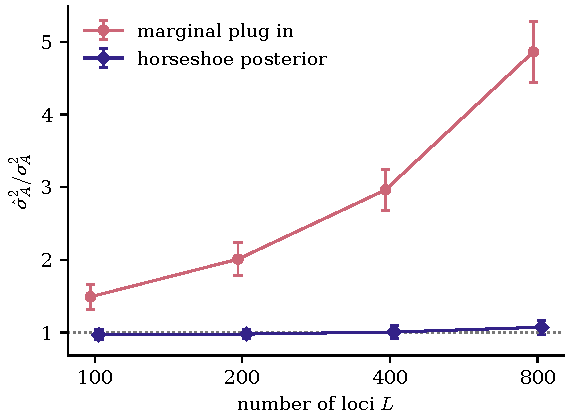
\includegraphics{figures/ftns_scaling.pdf}
\caption{Ratio of estimated to true additive variance in fitness as the number of genotyped loci grows with $n=300$ and the causal architecture held fixed. The naive estimator inflates linearly in $L$, as Proposition~\ref{hs:prop:bias} requires; the horseshoe posterior is flat. Error bars are $\pm2$ Monte Carlo standard errors over 6 replicates.}
\label{hs:fig:scaling}
\end{figure}

\begin{table}[t]
\centering
\small
\begin{adjustbox}{max width=\textwidth}
\begin{tabular}{@{}lccc@{}}
\toprule
Estimator & $\hat\sigma^2_A$ & $\hat\sigma^2_A/\sigma^2_A$ & MSE of $\hat\alpha$ \\
\midrule
truth & $0.0205$ & $1.00$ & $\cdot$ \\
marginal plug in & $0.0635$ & $3.24$ & $2.97\times10^{-4}$ \\
ridge (CV) & $0.0083$ & $0.40$ & $7.78\times10^{-5}$ \\
horseshoe plug in & $0.0186$ & $0.91$ & $1.51\times10^{-5}$ \\
horseshoe posterior & $0.0219$ & $1.08$ & $1.51\times10^{-5}$ \\
\bottomrule
\end{tabular}
\end{adjustbox}
\caption{Estimation of the additive genetic variance in fitness, $L=400$, $n=300$, 12 replicates; the third column averages the ratio over replicates, so it is not the ratio of the averages in the second. The implied rate of adaptation is $\hat\sigma^2_A/\bar w$ with $\bar w = 1$, so the third column is also the factor by which each method overstates or understates the rate.}
\label{hs:tab:sim}
\end{table}

\begin{figure}[t]
\centering
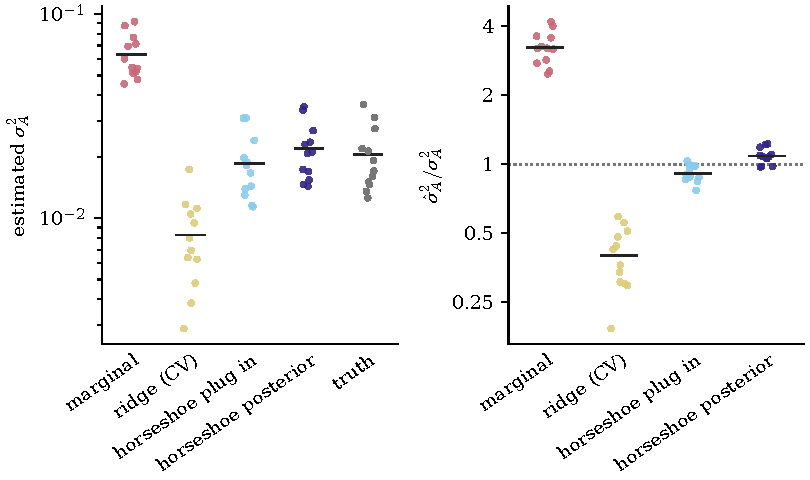
\includegraphics{figures/ftns_variance.pdf}
\caption{Left: estimated additive genetic variance in fitness across replicates, log scale. Right: ratio to the truth, log scale; the dotted line is exact recovery. The marginal estimator overstates roughly threefold, ridge understates substantially, and the two horseshoe estimators lie close to the truth, the plug in slightly below it and the posterior mean slightly above.}
\label{hs:fig:variance}
\end{figure}

\begin{figure}[t]
\centering
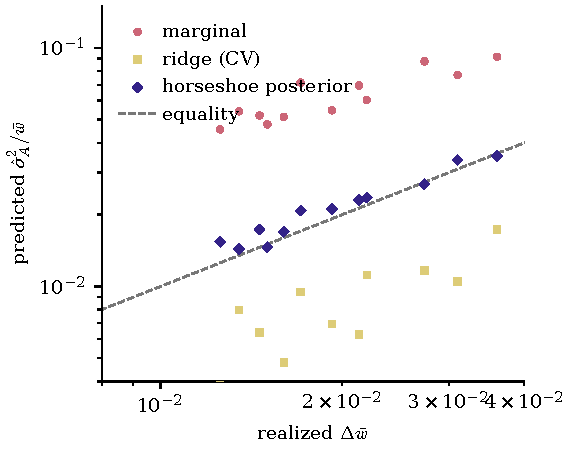
\includegraphics{figures/ftns_rate.pdf}
\caption{Rate of adaptation implied by the Fundamental Theorem, predicted against realized, across replicates. The dashed line is equality.}
\label{hs:fig:rate}
\end{figure}

\begin{figure}[t]
\centering
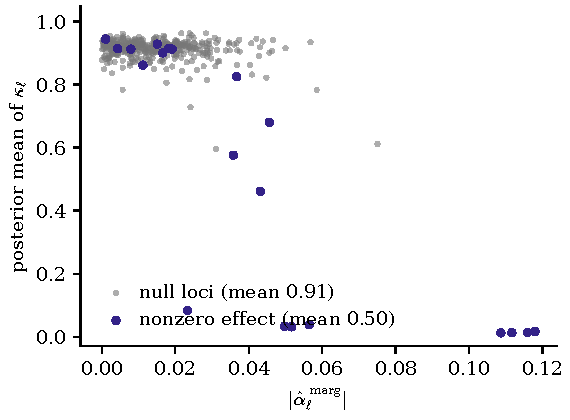
\includegraphics{figures/ftns_shrinkage.pdf}
\caption{Horseshoe shrinkage weights $\kappa_\ell$ against the magnitude of the marginal estimate, one replicate. Null loci have weights near one, so their estimates are shrunk almost to zero; loci with nonzero average effect have weights spread over the whole interval, and on average retain about half their marginal magnitude. The legend gives the mean weight in each group for this replicate.}
\label{hs:fig:shrinkage}
\end{figure}

\section{Robertson's secondary theorem and selection gradients}
\label{hs:sec:secondary}

The argument extends directly to two neighbouring results, in both of which the overparameterization is worse.

\emph{The secondary theorem.} Robertson's result \citep{hs:robertson1966mathematical} states that the change in the mean of any character $z$ equals the additive genetic covariance between $z$ and relative fitness. Written out, this replaces the quadratic form $\sum_\ell h_\ell \alpha_\ell^2$ by the bilinear form $\sum_\ell h_\ell \alpha_\ell \beta_\ell$, where $\beta_\ell$ are the average effects on the character. Both vectors must be estimated from the same overparameterized regression, and the product of two noisy estimates has a bias that depends on the correlation of their errors, a correlation that is present whenever the same individuals are used for both, as they invariably are. A horseshoe treatment shrinks both vectors and, because the shrinkage weights are locus specific, damps the spurious covariance contributed by null loci more aggressively than the genuine covariance at signal loci. Whether the bilinear analogue of Proposition~\ref{hs:prop:posterior} suffices to correct the resulting attenuation is a question I leave open; the required object is the posterior mean of a bilinear functional, $\sum_\ell h_\ell(m^\alpha_\ell m^\beta_\ell + \mathrm{Cov}(\alpha_\ell,\beta_\ell \mid y))$, and Section~\ref{hs:sec:open} returns to it.

The secondary theorem is the same least squares identity as Proposition~\ref{hs:prop:ftns}, with one of the two factors replaced. At a single locus, let the character have genotypic values $z_{ij} = z_{ji}$, mean $\bar z = \sum_{i,j}p_ip_jz_{ij}$, marginal values $z_i = \sum_jp_jz_{ij}$ and average effects $\beta_i = z_i - \bar z$, obtained from the regression \eqref{hs:eq:wls} with $z$ in place of $w$. Define the additive genetic covariance $\sigma_A(w,z) = 2\sum_ip_i\alpha_i\beta_i$ and the partial change $\Delta_\beta\bar z = 2\sum_i\beta_i\Delta p_i$.

\begin{proposition}[Secondary theorem]
\label{hs:prop:robertson}
Under the recursion \eqref{hs:eq:recursion}, $\Delta_\beta\bar z = \sigma_A(w,z)/\bar w$.
\end{proposition}

\begin{proof}
By \eqref{hs:eq:recursion}, $\Delta p_i = p_i(w_i-\bar w)/\bar w = p_i\alpha_i/\bar w$. Hence $2\sum_i\beta_i\Delta p_i = (2/\bar w)\sum_ip_i\alpha_i\beta_i = \sigma_A(w,z)/\bar w$.
\end{proof}

Setting $z = w$ recovers Proposition~\ref{hs:prop:ftns}, and the multilocus form under linkage equilibrium is $\sigma_A(w,z) = \sum_\ell h_\ell\alpha_\ell\beta_\ell$ with $\alpha_\ell,\beta_\ell$ the substitution effects. The interpretation is that a character responds to selection only through the part of its genetic variation that is linearly aligned with the genetic variation in fitness.

\begin{example}[Secondary theorem at one locus]
\label{hs:ex:robertson}
Keep the locus of Example~\ref{hs:ex:onelocus} and attach a character with genotypic values $z_{11} = 12$, $z_{12} = 11$, $z_{22} = 9$. Then $\bar z = 0.04(12) + 0.32(11) + 0.64(9) = 9.76$, $z_1 = 11.2$, $z_2 = 9.4$, and $\beta_1 = 1.44$, $\beta_2 = -0.36$. The additive covariance is
\[
\sigma_A(w,z) = 2\big[0.2(0.0448)(1.44) + 0.8(-0.0112)(-0.36)\big] = 0.032256,
\]
equal to $h(\alpha_1-\alpha_2)(\beta_1-\beta_2) = 0.32(0.056)(1.8)$. The secondary theorem predicts $\Delta_\beta\bar z = 0.032256/1.0232 = 0.031525$; evaluating $\bar z$ at $p_1' = 0.2087568$ gives an exact change of $0.031448$, so the partial change is again within a quarter of a percent of the total. The character rises because the allele that raises it also raises fitness, and by exactly the amount its additive covariance with fitness permits.
\end{example}

\emph{Selection gradients.} The Lande Arnold decomposition \citep{hs:lande1983measurement} estimates directional selection gradients as $\beta = P^{-1}s$, the coefficients of a multiple regression of relative fitness on phenotypic traits. With more traits than individuals, or with the near collinearity endemic to morphometric data, $P$ is ill conditioned and $P^{-1}s$ is unstable in exactly the way Section~\ref{hs:sec:bias} describes. The known pathologies, gradients that flip sign when a trait is added, quadratic terms that cannot be estimated at all, the well documented failure of the breeder's equation in observational settings \citep{hs:morrissey2010danger}, are the familiar symptoms of an overparameterized regression, and the standard remedies apply. A horseshoe prior on the gradient vector, or a regularized horseshoe variant when $P$ is badly conditioned, would deliver stable gradients with honest intervals, and is in my view a more promising route than the dimension reduction schemes currently used, which change the estimand without saying so.


\emph{Evolvability.} \citet{hs:houle1992comparing} argued that additive variances should be mean standardized before comparison, defining the evolvability $I_A = \sigma^2_A/\bar w^2$. In these terms Proposition~\ref{hs:prop:ftns} reads $\Delta \log \bar w \approx I_A$: the proportional rate of increase of mean fitness is the mean standardized additive variance. Every statement above transfers, since the standardization is a fixed scalar; but it is worth noting that comparative claims about evolvability across species or populations, which is what $I_A$ was introduced for, inherit the bias of Proposition~\ref{hs:prop:bias} in a form that does not cancel, because different studies genotype different numbers of loci at different sample sizes. Cross study comparisons of evolvability computed from plug in estimates are comparisons of $L/n$ as much as of biology.

\section{Four problems, addressed}
\label{hs:sec:open}

The propositions of Section~\ref{hs:sec:hs} leave four questions unresolved: the calibration of posterior intervals for a quadratic functional; the bilinear analogue required by the secondary theorem; the behaviour of the estimator under linkage disequilibrium; and the effect of ascertainment. This section takes each in turn. One is largely resolved, one is partially resolved, one is resolved in a way that revises the definition of the estimand, and one is not resolved at all, the last being, I think, the most useful of the four findings. Table~\ref{hs:tab:open} at the end of the section summarizes the status of each.

\subsection{Calibration of the posterior for the quadratic functional}

The coverage figure of Section~\ref{hs:sec:sim}, $83\%$ against a nominal $90\%$, was based on twelve replicates and therefore carried a Monte Carlo standard error of about $0.11$: it was not evidence of anything. Repeating the exercise with sixty replicates gives $85.0\%$ (standard error $4.6\%$) for the plain horseshoe and $90.0\%$ ($3.9\%$) for the regularized horseshoe of \citet{hs:piironen2017sparsity}. The plain prior is about one standard error below nominal and the regularized prior is at nominal. The shortfall of the plain prior is modest, and sixty replicates cannot distinguish it from none; the six hundred replicates of Remark~\ref{hs:rem:rerun} can ($84.8\%$, standard error $1.5\%$).

More informative than the coverage rate is the direction of the failures. Of the sixty intervals from the plain horseshoe, $13.3\%$ lay entirely \emph{above} the truth and only $1.7\%$ entirely below; for the regularized version, $5.0\%$ and $5.0\%$. Figure~\ref{hs:fig:coverage} shows these intervals. The misses of the plain horseshoe fall mostly above the truth, which fits the upward bias of its posterior mean (a mean ratio of $1.056$ in this experiment, $1.08$ in Table~\ref{hs:tab:sim}) and is the opposite of the direction that the theory of intermediate signals suggests. \citet{hs:vanderpas2017uncertainty} show that horseshoe credible sets are honest for signals that are either negligible or strong, and can fail for signals of intermediate size, which the prior shrinks more than the data warrant. The additive variance in fitness is a sum of squares dominated by precisely those intermediate loci, so on that argument the residual overshrinkage would accumulate in one direction and the interval would sit low. This run does not show it, and neither do nine further runs of the same size (Remark~\ref{hs:rem:rerun}).

Two practical conclusions follow. The regularized horseshoe should be preferred here: it improves both the coverage and the point estimate, returning a mean ratio of $1.021$ against $1.056$. And any reported interval for a rate of adaptation should be treated as having an effective level a few points below its nominal one; for the plain horseshoe the misses in this design err towards overstating $\sigma^2_A$ (Remark~\ref{hs:rem:rerun}).

\begin{remark}[How much can sixty intervals say?]
\label{hs:rem:rerun}
With sixty replicates and coverage of $85\%$ there are only nine misses in all, so the split between misses below and above the truth in one run rests on a handful of intervals. To settle the direction I repeated the experiment on nine further batches of sixty replicates with fresh seeds, giving $600$ intervals for each prior, the first batch being the one in Figure~\ref{hs:fig:coverage}. The plain horseshoe covers $509$ of $600$ ($84.8\%$, standard error $1.5\%$). Of its $91$ misses, $80$ lie entirely above the truth and $11$ entirely below, and every one of the ten batches has more misses above than below. In this design the direction is therefore stable: plain horseshoe intervals sit high, in line with the upward bias of its posterior mean (a mean ratio of $1.060$ over the $600$ replicates), and not low as the argument from intermediate signals suggests. The regularized horseshoe covers $536$ of $600$ ($89.3\%$, standard error $1.3\%$), with $39$ misses above and $25$ below; six batches have more misses above, two more below and two are tied, so its misses are much closer to balanced. Whether the upward direction persists in other architectures, sample sizes and priors on the global scale is not settled by this design.
\end{remark}

\begin{figure}[t]
\centering
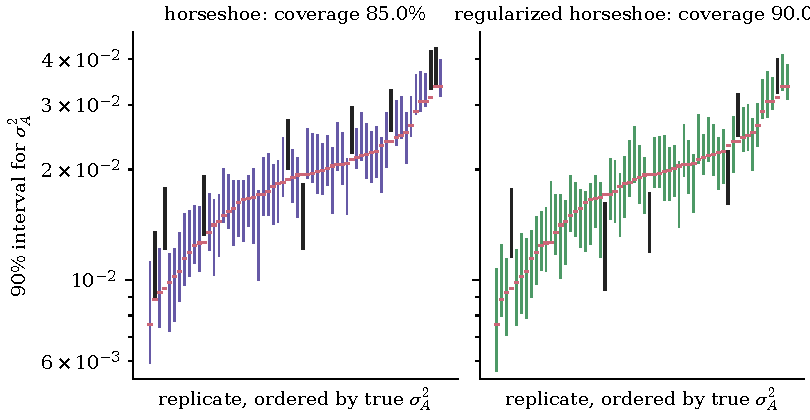
\includegraphics{figures/ftns_coverage.pdf}
\caption{Nominal $90\%$ posterior intervals for $\sigma^2_A$ across sixty replicates, ordered by the true value (short horizontal marks). Intervals that miss are drawn in black, and the empirical coverage of each prior is printed above its panel. These are the sixty replicates summarized in the text, the first of the ten batches of Remark~\ref{hs:rem:rerun}; the number of misses of the plain horseshoe varies between batches from $3$ to $13$, but in every batch most of them lie above the truth.}
\label{hs:fig:coverage}
\end{figure}

\subsection{The secondary theorem and the bilinear functional}

Robertson's theorem requires $\sigma_A(w,z) = \sum_\ell h_\ell \alpha_\ell\beta_\ell$, where $\alpha$ and $\beta$ are the average effects on fitness and on the character. Both are estimated from regressions on the same individuals, so their errors are correlated, and the plug in inherits a bias that the univariate analysis does not exhibit.

\begin{proposition}[Bias of the bilinear plug in]
\label{hs:prop:bilinear}
Let $y_w = X\alpha + \varepsilon_w$ and $y_z = X\beta + \varepsilon_z$ on the same $n$ individuals with $\mathrm{Corr}(\varepsilon_w,\varepsilon_z) = \rho$ and marginal standard deviations $\sigma_w,\sigma_z$. Under the orthogonality of Proposition~\ref{hs:prop:bias},
\[
\mathbb{E}\Big[\sum_\ell h_\ell \hat\alpha^{\rm marg}_\ell\hat\beta^{\rm marg}_\ell\Big]
= \sigma_A(w,z) + \frac{L\,\rho\,\sigma_w\sigma_z}{n}.
\]
\end{proposition}

\begin{proof}
Assume, as is implicit, that the pairs $(\varepsilon_{w,i},\varepsilon_{z,i})$ are uncorrelated across individuals. As in the proof of Proposition~\ref{hs:prop:bias}, $\hat\alpha^{\rm marg}_\ell = \alpha_\ell + e_\ell$ and $\hat\beta^{\rm marg}_\ell = \beta_\ell + f_\ell$ with $e_\ell = x_\ell^\top\varepsilon_w/(nh_\ell)$ and $f_\ell = x_\ell^\top\varepsilon_z/(nh_\ell)$, both of mean zero. Then
\[
\mathbb{E}\big[\hat\alpha^{\rm marg}_\ell\hat\beta^{\rm marg}_\ell\big] = \alpha_\ell\beta_\ell + \mathbb{E}[e_\ell f_\ell]
= \alpha_\ell\beta_\ell + \frac{x_\ell^\top\,\mathrm{Cov}(\varepsilon_w,\varepsilon_z)\,x_\ell}{(nh_\ell)^2}
= \alpha_\ell\beta_\ell + \frac{\rho\sigma_w\sigma_z\,nh_\ell}{(nh_\ell)^2},
\]
since $\mathrm{Cov}(\varepsilon_w,\varepsilon_z) = \rho\sigma_w\sigma_zI_n$. Multiplying by $h_\ell$ gives $h_\ell\alpha_\ell\beta_\ell + \rho\sigma_w\sigma_z/n$, and summing over the $L$ loci gives the result.
\end{proof}

For a sense of scale, take $L = 300$ loci, $n = 250$ individuals, a residual correlation $\rho = 0.5$, fitness residual standard deviation $\sigma_w = 0.1$ and a character measured in units of its residual standard deviation, $\sigma_z = 1$. The bias is $300(0.5)(0.1)(1)/250 = 0.06$. Unlike the quadratic case the bias can have either sign, since it takes the sign of $\rho$, so the plug in can manufacture a predicted response of the character in a direction the genetics does not support. A Monte Carlo check of the proposition on an orthogonal design with $L = 40$, $n = 64$ reproduces the predicted mean to three significant figures.

The structure mirrors Proposition~\ref{hs:prop:bias} with $\sigma^2_\varepsilon$ replaced by the residual covariance, and the bias vanishes only if the two residuals are uncorrelated, which they are not, since environmental effects on fitness and on a character measured in the same organism are correlated by construction, and since each residual also contains the signal of the loci not being tested, which are shared. In practice the effective $\rho$ differs from the environmental correlation for this second reason, by an amount that depends on the genetic correlation between fitness and the character.

The coherent estimator is the posterior mean of the bilinear functional,
\begin{equation}
\mathbb{E}\big[\sigma_A(w,z)\mid y\big] = \sum_\ell h_\ell\Big(m^\alpha_\ell m^\beta_\ell + \mathrm{Cov}(\alpha_\ell,\beta_\ell\mid y)\Big),
\label{hs:eq:bilinear}
\end{equation}
which requires a joint posterior over the two effect vectors. I use a bivariate horseshoe in which the two locus specific effects share a local scale,
\[
(\alpha_\ell,\beta_\ell)^\top \mid \lambda_\ell,\tau \ \sim\ N_2\big(0,\ \tau^2\lambda_\ell^2\,\mathrm{diag}(c_w,c_z)\big),
\qquad \lambda_\ell \sim C^{+}(0,1),
\]
with $c_w = \sigma_w^2(1-\rho^2)$ and $c_z = \sigma_z^2(1-\rho^2)$ the conditional residual variances, and the residual covariance $\Sigma_\varepsilon$ also estimated. Sharing $\lambda_\ell$ encodes the substantive belief that a locus is either relevant to both fitness and the character or to neither, which is the sparsity pattern the secondary theorem is about. Sampling proceeds by two conditional draws per sweep, each an ordinary horseshoe update on a residual adjusted response, so the fast sampler of Section~\ref{hs:sec:hs} applies unchanged; details are in Section~\ref{hs:app:gibbs}.

In simulation ($L = 300$, $n = 250$, twenty loci affecting both, residual correlation $0.5$, twelve replicates) the marginal plug in returns $2.58$ times the true genetic covariance. The bivariate horseshoe plug in returns $0.77$ and the posterior form \eqref{hs:eq:bilinear} returns $0.83$: the posterior covariance term supplies part of what the plug in loses, as in the univariate case, but not all of it. Figure~\ref{hs:fig:secondary} shows the distributions. A residual attenuation of about $17\%$ remains, and I do not have a correction for it; the shrinkage of two correlated vectors interacts in a way the univariate argument of Proposition~\ref{hs:prop:oracle} does not capture. What can be said is that the bilinear estimator is wrong by seventeen percent in the conservative direction where the standard estimator is wrong by a factor of two and a half in the anticonservative one.

\begin{figure}[t]
\centering
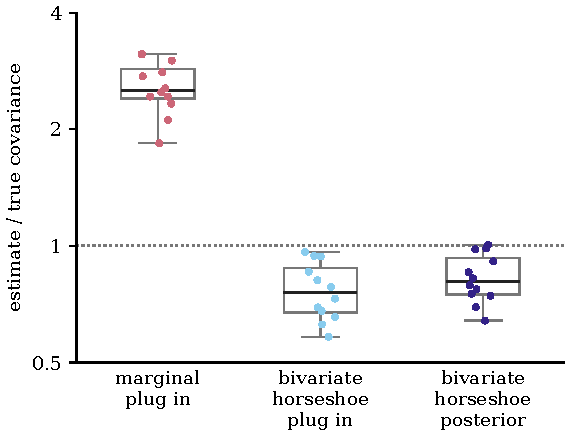
\includegraphics{figures/ftns_secondary.pdf}
\caption{Estimation of the additive genetic covariance between fitness and a character, twelve replicates, log scale. The marginal plug in overstates by a factor of about two and a half; both bivariate horseshoe estimators understate moderately, the posterior form less than the plug in.}
\label{hs:fig:secondary}
\end{figure}

\subsection{Linkage disequilibrium changes the functional, not just the estimator}

The formula $\sigma^2_A = \sum_\ell h_\ell\alpha_\ell^2$ of \eqref{hs:eq:s2A} assumes linkage equilibrium. In general the additive genetic variance is the variance of the breeding value $\sum_\ell \alpha_\ell g_\ell$, so
\begin{equation}
\sigma^2_A = \alpha^\top V \alpha, \qquad V = \mathrm{Var}(g),
\label{hs:eq:quadform}
\end{equation}
with $V$ reducing to $\mathrm{diag}(h)$ only under equilibrium. This is not a refinement of the estimator; it is a different estimand, and using the diagonal form when $V$ is not diagonal discards the covariance between the breeding value contributions of linked loci. Propositions~\ref{hs:prop:bias} and \ref{hs:prop:posterior} generalize cleanly.

\begin{proposition}[General quadratic form]
\label{hs:prop:ld}
Under \eqref{hs:eq:quadform}, the ordinary least squares plug in satisfies
\[
\mathbb{E}\big[\hat\alpha^\top V\hat\alpha\big] = \sigma^2_A + \sigma^2_\varepsilon\,\mathrm{tr}\big(V (X^\top X)^{-1}\big),
\]
and the posterior mean of the functional is $\mathbb{E}[\sigma^2_A\mid y] = m^\top V m + \mathrm{tr}\big(V\,\mathrm{Cov}(\alpha\mid y)\big)$.
\end{proposition}

\begin{proof}
$\mathbb{E}[\hat\alpha^\top V \hat\alpha] = \alpha^\top V\alpha + \mathrm{tr}(V\,\mathrm{Var}(\hat\alpha))$ with $\mathrm{Var}(\hat\alpha) = \sigma^2_\varepsilon (X^\top X)^{-1}$; the posterior statement is the same identity applied to the posterior distribution.
\end{proof}

Under orthogonality with $V = \mathrm{diag}(h)$ and $X^\top X = n\,\mathrm{diag}(h)$, the trace is $L/n$ and Proposition~\ref{hs:prop:bias} is recovered; with $V$ replaced by the sample covariance $X^\top X/n$ the trace is $L/n$ for every design, which is Proposition~\ref{hs:prop:biasols}; so \eqref{hs:eq:quadform} is the general statement of which the earlier result is the equilibrium special case.

Simulation with block linkage disequilibrium (blocks of ten, within block latent correlation $0.8$, which gives a mean sample correlation of $0.58$ between dosages in the same block, $L = 400$, $n = 300$, sixty replicates) bears out the first half of this argument and qualifies the second. The marginal plug in with diagonal weights returns $6.22$ times the truth, far worse than the $3.24$ of the equilibrium case, because LD tagging and overfitting compound as Section~\ref{hs:sec:bias} argues. The horseshoe plug in with diagonal weights returns $0.80$, and the same plug in with the full form $m^\top Vm$ returns $0.90$: shrinkage removes the overfitting, and the diagonal form then loses a further nine percent of the truth (a paired difference of $0.09$, Monte Carlo standard error $0.02$), because the posterior mean spreads each causal effect over the loci that tag it and the diagonal form discards their positive cross products. The posterior mean of the functional returns $1.02$ with diagonal weights and $1.00$ with the full form $\alpha^\top V\alpha$, so for the coherent estimator the choice of functional matters little here. That is a property of this design rather than a general reassurance: the twenty causal loci rarely share a block, so the diagonal form of the true effects averages $1.01$ times $\alpha^\top V\alpha$, whereas when causal loci share blocks the cross terms $2\sum_{\ell<m}V_{\ell m}\alpha_\ell\alpha_m$ need not vanish in a given population and the diagonal form is wrong at the truth itself. The lesson is that under LD the estimand is $\alpha^\top V\alpha$, and that a plug in which fixes the estimator but keeps diagonal weights adds a systematic error of the same order as the overshrinkage of the plug in itself.

\subsection{Ascertainment is not a shrinkage problem}

Fitness is not measured on a random sample. It is measured on the individuals who survived long enough to be measured, which is selection on the very variable being analysed. To gauge the effect I repeated the base simulation with $n = 400$ (sixty replicates), then discarded the lower half of the population by realized fitness and reestimated from the survivors alone.

The result is stark. On the full sample the horseshoe posterior returns $1.03$ times the true additive variance (Monte Carlo standard error $0.01$). On the truncated sample it returns $0.27$ (standard error $0.02$), and rescaling by the ratio of genotypic variances between the two samples (the obvious first aid correction) barely moves it, to $0.28$. Truncating on the dependent variable attenuates every regression coefficient, and squaring the attenuated coefficients attenuates the additive variance roughly quadratically. An almost fourfold understatement swamps the twofold to sixfold overstatement that shrinkage was introduced to fix, and it runs in the opposite direction, so the two errors partially cancel in a way that is entirely accidental and cannot be relied upon.

This is a negative result and I state it plainly: no shrinkage prior addresses this. Ascertainment is a bias in the estimand, not variance in the estimator, and the two are orthogonal problems. The remedy has to come from the likelihood (a truncated or selection corrected model of the sampling, in the tradition of Heckman type corrections, with the selection rule modelled explicitly) and only then does the shrinkage question arise, on the corrected likelihood. Since almost all fitness data in natural populations are ascertained in some such way, I would put this ahead of everything else in Section~\ref{hs:sec:hs} as the practically binding constraint on estimating rates of adaptation. It is also, unlike the others, not a statistical problem that can be solved by a better prior.

\subsubsection*{An exact calculation for truncation selection}

The size of the ascertainment effect can be computed exactly in a Gaussian version of the problem, and the calculation shows both why the damage is so large and why the cure has to come from the likelihood. Let the centred dosage vector $x \in \mathbb{R}^L$ have covariance $V$, let $y = x^\top\alpha + \varepsilon$ with $\varepsilon$ independent of $x$ and of variance $\sigma^2_\varepsilon$, and write $\sigma^2_A = \alpha^\top V\alpha$, $V_y = \sigma^2_A + \sigma^2_\varepsilon$ and $R^2 = \sigma^2_A/V_y$ for the proportion of the measured variance that is additive. Suppose $(x,y)$ is jointly Gaussian, which is accurate for the breeding value when many loci each contribute a little, and that only individuals with $y > c$ are measured, a fraction $q$ of the population. Put $c' = (c - \mathbb{E}y)/\sqrt{V_y}$, $\lambda = \phi(c')/q$ with $\phi$ the standard normal density, and
\[
\delta = \lambda(\lambda - c') \in (0,1),
\]
the proportional reduction in the variance of a standard normal truncated below at $c'$.

\begin{proposition}[Truncation on measured fitness]
\label{hs:prop:trunc}
Among the measured individuals, the regression coefficients of $y$ on $x$ are
\[
\alpha_S = \frac{1-\delta}{1-\delta R^2}\,\alpha,
\]
and the additive variance computed from them is
\[
\alpha_S^\top V_S\,\alpha_S = \frac{(1-\delta)^2}{1-\delta R^2}\,\sigma^2_A
\qquad\text{or}\qquad
\alpha_S^\top V\alpha_S = \Big(\frac{1-\delta}{1-\delta R^2}\Big)^2\sigma^2_A ,
\]
according as the genotypic covariance $V_S$ of the survivors or the covariance $V$ of the whole population is used.
\end{proposition}

\begin{proof}
Because $(x,y)$ is jointly Gaussian, $x = \mathbb{E}x + b\,(y - \mathbb{E}y) + u$ with $b = \mathrm{Cov}(x,y)/V_y = V\alpha/V_y$ and $u$ Gaussian, independent of $y$, with covariance $V - bb^\top V_y$. Selection on $y$ alone leaves the distribution of $u$ unchanged and $u$ independent of $y$. Among survivors, therefore, $\mathrm{Var}(y\mid S) = V_y(1-\delta)$ by the truncated normal variance formula, and
\begin{align*}
\mathrm{Cov}(x,y\mid S) &= b\,V_y(1-\delta) = (1-\delta)V\alpha,\\
V_S = \mathrm{Var}(x\mid S) &= V - bb^\top V_y + bb^\top V_y(1-\delta) = V - \frac{\delta}{V_y}V\alpha\alpha^\top V .
\end{align*}
The survivor regression coefficient is $\alpha_S = V_S^{-1}\mathrm{Cov}(x,y\mid S)$. To invert $V_S$ on the vector $V\alpha$, note that
\[
\Big(V - \frac{\delta}{V_y}V\alpha\alpha^\top V\Big)\alpha = V\alpha\Big(1 - \frac{\delta\,\alpha^\top V\alpha}{V_y}\Big) = (1-\delta R^2)\,V\alpha ,
\]
so $V_S^{-1}V\alpha = \alpha/(1-\delta R^2)$ and $\alpha_S = (1-\delta)\alpha/(1-\delta R^2)$. Finally $\alpha^\top V_S\alpha = \sigma^2_A - \delta\sigma^4_A/V_y = \sigma^2_A(1-\delta R^2)$, which, multiplied by the square of the scalar factor, gives the first form; the second is immediate.
\end{proof}

Every coefficient is attenuated by the same factor, so truncation does not distort which loci matter, only how much. This is why no prior can detect it: to a regression fitted on the survivors, a population with effects $\alpha$ seen through truncation looks exactly like an untruncated population with the smaller effects $\alpha_S$, and nothing in a prior on effect sizes can tell the two apart. The additive variance is attenuated by roughly the square of the factor, and rescaling to the population genotypic variance (the first aid correction mentioned above) changes only the denominator: it replaces $(1-\delta)^2/(1-\delta R^2)$ by $(1-\delta)^2/(1-\delta R^2)^2$ and leaves the dominant $(1-\delta)^2$ untouched.

\begin{example}[Discarding the less fit half]
\label{hs:ex:trunc}
If the lower half is discarded, $q = 1/2$, $c' = 0$, $\lambda = \phi(0)/0.5 = 0.7979$ and $\delta = \lambda^2 = 2/\pi = 0.6366$. With $R^2 = 0.5$ the coefficients shrink by the factor $0.3634/0.6817 = 0.533$; the additive variance computed on survivors is $0.194$ of the truth and the rescaled version $0.284$. For the setting of Section~\ref{hs:sec:sim}, where $\sigma^2_A = 0.0205$ out of a phenotypic variance of $0.0320$, so $R^2 \approx 0.64$, the large sample values are $0.223$ and $0.376$. The simulated horseshoe values reported above, $0.27$ and $0.28$, use the diagonal form $\sum_\ell h_\ell\alpha_\ell^2$, with survivor and population dosage variances respectively. The diagonal form misses the linkage disequilibrium that truncation induces among the causal loci, which lowers the variance of the breeding value but barely changes the dosage variance of any single locus, so both values should be compared with the second form of the proposition, whose limit at the simulation's own $R^2 = 0.62$ is $0.36$. They fall below it, which is plausible for $200$ survivors genotyped at $400$ loci, far from the large sample limit, where the overfitting of Proposition~\ref{hs:prop:bias} pushes upward and the prior's own shrinkage pushes downward; the simulation does not separate the two. With the full survivor covariance, the posterior mean of $\alpha^\top V_S\alpha$, the same fits return $0.22$ (standard error $0.01$), against a limit of $0.22$ from the first form. That agreement should not be read as a confirmation of the limit: the proposition puts the diagonal form above the full form by the factor $1/(1-\delta R^2) = 1.65$, whereas in the fits the ratio of the two averages is $1.21$, so the finite sample effects move the two forms differently. What the simulation does confirm is the size of the loss, roughly three quarters of the additive variance whichever form is used. Table~\ref{hs:tab:trunc} gives the factors over a range of truncation fractions and heritabilities of fitness. Even mild ascertainment, losing the least fit tenth, costs roughly forty to fifty percent of the additive variance computed on the survivors.

As a check, a simulation with $200$ independent biallelic loci and $400{,}000$ individuals, of whom the fitter half are kept, gives with $R^2 = 0.5$ a coefficient factor of $0.531$, a survivor ratio of $0.195$ and a rescaled ratio of $0.283$, against theoretical values $0.533$, $0.194$ and $0.284$; the binomial dosages are not Gaussian, but the breeding value summed over many loci is close enough.

The proposition also shows what a likelihood correction looks like. If the truncation fraction is known, $\delta$ is known, $V_y = \mathrm{Var}(y\mid S)/(1-\delta)$ is estimable from the survivors, and the first identity of the proposition can be solved for the target:
\[
\sigma^2_A = \frac{s_S}{(1-\delta)^2 + \delta\,s_S/V_y},
\qquad s_S = \alpha_S^\top V_S\,\alpha_S .
\]
In the same simulation this returns $1.003$ times the truth with $R^2 = 0.5$ and $1.008$ with $R^2 = 0.65$. The correction works because the selection rule was written into the model, as in the sample selection models of econometrics \citep{hs:heckman1979sample}. It depends entirely on knowing the selection rule; in a natural population where the measured survivors were selected on an unobserved combination of viability and fertility, the same algebra holds with an unknown $\delta$, and the data on survivors can recover it only through strong assumptions about the shape of the fitness distribution.
\end{example}

\begin{table}[t]
\centering
\small
\begin{tabular}{@{}cc cc cc cc@{}}
\toprule
& & \multicolumn{2}{c}{$R^2 = 0.1$} & \multicolumn{2}{c}{$R^2 = 0.5$} & \multicolumn{2}{c}{$R^2 = 0.65$} \\
\cmidrule(lr){3-4}\cmidrule(lr){5-6}\cmidrule(l){7-8}
kept, $q$ & $\delta$ & survivors & rescaled & survivors & rescaled & survivors & rescaled \\
\midrule
$0.90$ & $0.288$ & $0.522$ & $0.538$ & $0.592$ & $0.692$ & $0.624$ & $0.767$ \\
$0.75$ & $0.465$ & $0.300$ & $0.314$ & $0.373$ & $0.486$ & $0.410$ & $0.588$ \\
$0.50$ & $0.637$ & $0.141$ & $0.151$ & $0.194$ & $0.284$ & $0.225$ & $0.384$ \\
$0.25$ & $0.758$ & $0.063$ & $0.068$ & $0.094$ & $0.151$ & $0.115$ & $0.227$ \\
\bottomrule
\end{tabular}
\caption{Ratio of the additive variance estimated from survivors to the true additive variance under truncation selection on measured fitness, from Proposition~\ref{hs:prop:trunc}. ``Survivors'' uses the survivors' genotypic covariance, ``rescaled'' the population covariance; $R^2$ is the additive proportion of the variance in measured fitness.}
\label{hs:tab:trunc}
\end{table}

\begin{table}[t]
\centering
\small
\begin{tabularx}{\textwidth}{>{\raggedright\arraybackslash}p{1.2in}>{\raggedright\arraybackslash}X>{\raggedright\arraybackslash}X}
\toprule
Problem & Status & Numerical summary \\
\midrule
Coverage of $\sigma^2_A$ intervals & largely resolved; use the regularized horseshoe & $85.0\%$ plain, $90.0\%$ regularized in sixty replicates ($84.8\%$ and $89.3\%$ in $600$), nominal $90\%$; plain misses mostly above the truth ($80$ of $91$ in $600$ replicates) \\
Bilinear functional & partially resolved; bivariate prior with shared local scale & marginal $2.58\times$; bivariate posterior $0.83\times$ \\
Linkage disequilibrium & resolved by changing the estimand to $\alpha^\top V\alpha$ & horseshoe plug in, diagonal $0.80\times$, full $0.90\times$; posterior mean $1.00\times$; marginal $6.22\times$ \\
Ascertainment & not resolved; not a shrinkage problem & $1.03\times$ full sample, $0.27\times$ on survivors \\
\bottomrule
\end{tabularx}
\caption{Status of the four problems.}
\label{hs:tab:open}
\end{table}

\section{Discussion}

The Fundamental Theorem is exact and, in Ewens's formulation, clear. What it delivers, however, is a statement about a least squares quantity, and the difficulty of using it empirically is entirely the difficulty of estimating that quantity when there are more loci than individuals. The naive estimator overstates the rate of adaptation by a factor that grows linearly in the number of loci. Ridge type shrinkage overcorrects. A horseshoe prior, combined with the recognition that the additive variance is a quadratic functional requiring the posterior mean rather than the plug in, comes close to the truth in the simulations reported here.

Three caveats deserve emphasis. First, the choice of prior encodes a hypothesis about genetic architecture, and with $L>n$ the data cannot fully adjudicate it; sensitivity across prior families should be reported alongside any estimated rate. Second, the coverage of posterior intervals for the quadratic functional is a few points below nominal, and in $600$ replicates the misses of the plain horseshoe fall mostly above the truth (Remark~\ref{hs:rem:rerun}), so a reported interval for a rate of adaptation should be read as somewhat narrower than its nominal level warrants; the regularized horseshoe should be the default for this reason. Third, and most seriously, real fitness data are ascertained. Section~\ref{hs:sec:open} shows that measuring fitness on survivors alone can understate the additive variance almost fourfold, that this is a bias in the estimand rather than variance in the estimator, and that no choice of prior repairs it. Until the selection mechanism is written into the likelihood, the shrinkage question is secondary to it.

The broader point is that a century of interpretive dispute about the Fundamental Theorem was, in the end, a dispute about what quantity Fisher was regressing on what. Now that the question is settled, the remaining obstacle is not conceptual but statistical, and it is the same obstacle that afflicts every other high dimensional problem in genetics: too many parameters, too few individuals, and an estimator that mistakes noise for signal unless it is told not to.




\section{Posterior sampling}
\label{hs:app:gibbs}

The half Cauchy priors in \eqref{hs:eq:hs} are written as inverse gamma scale mixtures following \citet{hs:makalic2016simple}: if $\lambda^2 \mid \nu \sim \mathrm{IG}(1/2, 1/\nu)$ and $\nu \sim \mathrm{IG}(1/2,1)$, then $\lambda \sim C^{+}(0,1)$, and similarly for $\tau$ with auxiliary $\xi$. Every full conditional is then conjugate. With $D = \mathrm{diag}(\sigma^2_\varepsilon \tau^2\lambda_1^2,\ldots,\sigma^2_\varepsilon\tau^2\lambda_L^2)$ the sweep is

\begin{enumerate}\itemsep1pt
\item $\alpha \mid \cdot \ \sim\ N\big(A^{-1}\Phi^\top \tilde y,\ A^{-1}\big)$ with $\Phi = X/\sigma_\varepsilon$, $\tilde y = y/\sigma_\varepsilon$, $A = \Phi^\top\Phi + D^{-1}$;
\item $\sigma^2_\varepsilon \mid \cdot \ \sim\ \mathrm{IG}\big(\tfrac{n+L}{2},\ \tfrac12\|y-X\alpha\|^2 + \tfrac12\sum_\ell \alpha_\ell^2/(\tau^2\lambda_\ell^2)\big)$;
\item $\lambda_\ell^2 \mid \cdot \ \sim\ \mathrm{IG}\big(1,\ 1/\nu_\ell + \alpha_\ell^2/(2\tau^2\sigma^2_\varepsilon)\big)$ and $\nu_\ell \mid \cdot \sim \mathrm{IG}(1, 1+1/\lambda_\ell^2)$;
\item $\tau^2 \mid \cdot \ \sim\ \mathrm{IG}\big(\tfrac{L+1}{2},\ 1/\xi + \tfrac{1}{2\sigma^2_\varepsilon}\sum_\ell \alpha_\ell^2/\lambda_\ell^2\big)$ and $\xi \mid \cdot \sim \mathrm{IG}(1,1+1/\tau^2)$.
\end{enumerate}

Step 1 is executed by the algorithm of \citet{hs:bhattacharya2016fast}, which avoids forming $A$: draw $u \sim N(0,D)$ and $\delta \sim N(0,I_n)$, set $v = \Phi u + \delta$, solve $(\Phi D\Phi^\top + I_n)w = \tilde y - v$, and return $\alpha = u + D\Phi^\top w$. The cost is $O(n^2L)$ per iteration, so the sampler is cheapest exactly when $L > n$, which is the regime of interest. The bivariate sampler of Section~\ref{hs:sec:open} adds one step. Conditional on $\beta$, the fitness residual is regressed after adjusting for the character residual: with $r_z = y_z - X\beta$, the response $y_w - \rho(\sigma_w/\sigma_z) r_z$ follows an ordinary regression on $X$ with error variance $\sigma_w^2(1-\rho^2)$, so step 1 applies verbatim; the roles are then exchanged to draw $\beta$. The shared local scale is updated from both coefficients, $\lambda_\ell^2 \mid \cdot \sim \mathrm{IG}\big(3/2,\ 1/\nu_\ell + (\alpha_\ell^2/c_w + \beta_\ell^2/c_z)/(2\tau^2)\big)$ with $c_w,c_z$ the conditional variances, which is the two dimensional group horseshoe update. The residual covariance is refreshed from the current residuals each sweep.

All results in Section~\ref{hs:sec:sim} use 1200 iterations with the first 400 discarded; the additive variance is computed on each retained draw as $\sum_\ell h_\ell \alpha_\ell^2$, giving the posterior distribution required by Proposition~\ref{hs:prop:posterior} directly rather than by a delta method approximation.

\section{Exercises}
\label{hs:sec:exercises}

\begin{enumerate}[label=\arabic*.,leftmargin=*,itemsep=4pt]
\item\label{hs:exr:total} Show that the total genetic variance in fitness at one locus decomposes as $\sum_{i,j}p_ip_j(w_{ij}-\bar w)^2 = \sigma^2_A + \sigma^2_D$, and check it on Example~\ref{hs:ex:onelocus}.
\emph{Hint.} The normal equations say the residuals $r_{ij}$ are orthogonal, in the $p_ip_j$ weighted inner product, to the constant and to every $\alpha_i + \alpha_j$.

\item\label{hs:exr:twoallele} For two alleles with $w_{11} = m + a$, $w_{12} = m + d$, $w_{22} = m - a$ and $p = p_1$, show that $\alpha_1 - \alpha_2 = a + d(1-2p)$, $\sigma^2_A = 2p(1-p)\big[a + d(1-2p)\big]^2$ and $\sigma^2_D = \big[2p(1-p)d\big]^2$.
\emph{Hint.} Compute $w_1 - w_2$ directly; for $\sigma^2_D$ evaluate the residual at the heterozygote and use Exercise~\ref{hs:exr:total}.

\item\label{hs:exr:remainder} With the parameterization of Exercise~\ref{hs:exr:twoallele}, show that the exact one generation change is $\Delta\bar w = 2(\alpha_1-\alpha_2)\Delta p + (w_{11} - 2w_{12} + w_{22})(\Delta p)^2$, so that the remainder in \eqref{hs:eq:decomp} is $R = -2d(\Delta p)^2$. Verify $R = -7.5\times10^{-6}$ in Example~\ref{hs:ex:overdominance} at $q = 0.05$.
\emph{Hint.} $\bar w$ is a quadratic in $p$, so its second order Taylor expansion is exact, and $d\bar w/dp = 2(w_1 - w_2)$.

\item In Example~\ref{hs:ex:overdominance}, show that $w_A = w_S$, and hence $\sigma^2_A = 0$, exactly when $q = s/(s+t)$, and that $\sigma^2_D = \big[2q^*(1-q^*)\big]^2(s+t)^2/4$ there. Evaluate it.
\emph{Hint.} In the notation of Exercise~\ref{hs:exr:twoallele} the dominance deviation is $d = (s+t)/2$ relative to the homozygote midpoint.

\item Under the conditions of Proposition~\ref{hs:prop:bias} with Gaussian errors and $\alpha = 0$, show that $(n/\sigma^2_\varepsilon)\sum_\ell h_\ell(\hat\alpha^{\rm marg}_\ell)^2$ has a $\chi^2_L$ distribution, and deduce part (b) of the proposition in this case.
\emph{Hint.} In standardized units the statistic is $\sum_\ell z_\ell^2$ with independent standard normal $z_\ell$.

\item For the design of Table~\ref{hs:tab:small}, compute $(X^\top X)^{-1}$ and confirm that the variance inflation factors are $6, 3, 5, 3, 3$. Then draw $1000$ noise vectors with $\sigma_\varepsilon = 0.05$ and check the two expectations in Example~\ref{hs:ex:small}.
\emph{Hint.} The diagonal of $X^\top X$ is $4$ throughout, so $\mathrm{VIF}_\ell = 4\,[(X^\top X)^{-1}]_{\ell\ell}$.

\item Derive the density \eqref{hs:eq:kappaprior} of the shrinkage weight from $\lambda \sim C^+(0,1)$, and show it reduces to $\mathrm{Beta}(1/2,1/2)$ when $\tau = 1$.
\emph{Hint.} $\lambda = \tau^{-1}\sqrt{(1-\kappa)/\kappa}$ and $|d\lambda/d\kappa| = \tfrac12\tau^{-1}\kappa^{-3/2}(1-\kappa)^{-1/2}$.

\item Prove \eqref{hs:eq:gap} using the law of total variance applied to $\theta_\ell$ given $z_\ell$, conditioning on $\kappa_\ell$.
\emph{Hint.} $\mathrm{Var}(\theta\mid z) = \mathbb{E}[\mathrm{Var}(\theta\mid z,\kappa)\mid z] + \mathrm{Var}(\mathbb{E}[\theta\mid z,\kappa]\mid z)$.

\item (Ridge as a common weight.) Suppose a single weight $\kappa$ is applied to every locus, $\hat\theta_\ell = (1-\kappa)z_\ell$. Show that the weight minimizing $\mathbb{E}\sum_\ell(\hat\theta_\ell - \theta_\ell)^2$ is $\kappa^* = L/(\|\theta\|^2 + L)$ and that $\mathbb{E}\sum_\ell\hat\theta_\ell^2 = \|\theta\|^4/(\|\theta\|^2+L)$ at this weight. Deduce that when $\|\theta\|^2 = L/2$ oracle ridge recovers one third of the additive variance, and compare with Proposition~\ref{hs:prop:oracle}.
\emph{Hint.} Repeat the proof of Proposition~\ref{hs:prop:oracle} with the sums over loci taken before minimizing.

\item In the bivariate sampler of Section~\ref{hs:app:gibbs}, show that conditional on $\beta$ the adjusted response $y_w - \rho(\sigma_w/\sigma_z)(y_z - X\beta)$ equals $X\alpha$ plus Gaussian noise of variance $\sigma_w^2(1-\rho^2)$, independent across individuals.
\emph{Hint.} Use the conditional distribution of $\varepsilon_w$ given $\varepsilon_z$ for a bivariate normal pair.

\item Verify that $\delta = 2/\pi$ when the lower half is discarded, and use Proposition~\ref{hs:prop:trunc} to reproduce the row $q = 0.75$ of Table~\ref{hs:tab:trunc}. What fraction must be kept for the survivors' additive variance to be at least $90\%$ of the truth when $R^2 = 0.5$?
\emph{Hint.} $c' = \Phi^{-1}(1-q)$; solve $(1-\delta)^2/(1-\delta R^2) = 0.9$ for $\delta$ and then for $q$ numerically.

\item (Computation.) Simulate $n = 200$ individuals at $L = 50, 100, 200, 400, 800$ independent loci with twenty causal loci of fixed effect, compute the marginal plug in, and plot its excess over $\sigma^2_A$ against $L$. Fit a line through the origin and compare its slope with $\sigma^2_y/n$.
\emph{Hint.} For the marginal estimator the effective error variance of each single locus regression is the phenotypic variance, which includes the signal of the other loci.
\end{enumerate}

\begin{small}
\setlength{\bibsep}{0.6pt}
\begin{thebibliography}{99}
\footnotesize
\bibitem[Barton et al.(2017)]{hs:barton2017infinitesimal} Barton, N.\ H., Etheridge, A.\ M.\ and V\'eber, A. (2017). The infinitesimal model: definition, derivation, and implications. \emph{Theoretical Population Biology} 118, 50 to 73.
\bibitem[Bhadra et al.(2019)]{hs:bhadra2019lasso} Bhadra, A., Datta, J., Polson, N.\ G.\ and Willard, B. (2019). Lasso meets horseshoe: a survey. \emph{Statistical Science} 34, 405 to 427.
\bibitem[Bhattacharya et al.(2016)]{hs:bhattacharya2016fast} Bhattacharya, A., Chakraborty, A.\ and Mallick, B.\ K. (2016). Fast sampling with Gaussian scale mixture priors in high dimensional regression. \emph{Biometrika} 103, 985 to 991.
\bibitem[Carvalho et al.(2010)]{hs:carvalho2010horseshoe} Carvalho, C.\ M., Polson, N.\ G.\ and Scott, J.\ G. (2010). The horseshoe estimator for sparse signals. \emph{Biometrika} 97, 465 to 480.
\bibitem[Datta and Ghosh(2013)]{hs:datta2013asymptotic} Datta, J.\ and Ghosh, J.\ K. (2013). Asymptotic properties of Bayes risk for the horseshoe prior. \emph{Bayesian Analysis} 8, 111 to 132.
\bibitem[Edwards(1994)]{hs:edwards1994fundamental} Edwards, A.\ W.\ F. (1994). The fundamental theorem of natural selection. \emph{Biological Reviews} 69, 443 to 474.
\bibitem[Ewens(1989)]{hs:ewens1989interpretation} Ewens, W.\ J. (1989). An interpretation and proof of the fundamental theorem of natural selection. \emph{Theoretical Population Biology} 36, 167 to 180.
\bibitem[Ewens(2004)]{hs:ewens2004mathematical} Ewens, W.\ J. (2004). \emph{Mathematical Population Genetics I: Theoretical Introduction}, 2nd ed. Springer.
\bibitem[Ewens and Lessard(2015)]{hs:ewens2015interpretation} Ewens, W.\ J.\ and Lessard, S. (2015). On the interpretation and relevance of the fundamental theorem of natural selection. \emph{Theoretical Population Biology} 104, 59 to 67.
\bibitem[Fisher(1918)]{hs:fisher1918correlation} Fisher, R.\ A. (1918). The correlation between relatives on the supposition of Mendelian inheritance. \emph{Transactions of the Royal Society of Edinburgh} 52, 399 to 433.
\bibitem[Fisher(1930)]{hs:fisher1930genetical} Fisher, R.\ A. (1930). \emph{The Genetical Theory of Natural Selection}. Clarendon Press, Oxford.
\bibitem[Frank and Slatkin(1992)]{hs:frank1992fishers} Frank, S.\ A.\ and Slatkin, M. (1992). Fisher's fundamental theorem of natural selection. \emph{Trends in Ecology and Evolution} 7, 92 to 95.
\bibitem[Heckman(1979)]{hs:heckman1979sample} Heckman, J.\ J. (1979). Sample selection bias as a specification error. \emph{Econometrica} 47, 153 to 161.
\bibitem[Hill et al.(2008)]{hs:hill2008data} Hill, W.\ G., Goddard, M.\ E.\ and Visscher, P.\ M. (2008). Data and theory point to mainly additive genetic variance for complex traits. \emph{PLoS Genetics} 4, e1000008.
\bibitem[Houle(1992)]{hs:houle1992comparing} Houle, D. (1992). Comparing evolvability and variability of quantitative traits. \emph{Genetics} 130, 195 to 204.
\bibitem[Lande and Arnold(1983)]{hs:lande1983measurement} Lande, R.\ and Arnold, S.\ J. (1983). The measurement of selection on correlated characters. \emph{Evolution} 37, 1210 to 1226.
\bibitem[Lessard(1997)]{hs:lessard1997fisher} Lessard, S. (1997). Fisher's fundamental theorem of natural selection revisited. \emph{Theoretical Population Biology} 52, 119 to 136.
\bibitem[Makalic and Schmidt(2016)]{hs:makalic2016simple} Makalic, E.\ and Schmidt, D.\ F. (2016). A simple sampler for the horseshoe estimator. \emph{IEEE Signal Processing Letters} 23, 179 to 182.
\bibitem[Maynard Smith and Haigh(1974)]{hs:smith1974hitch} Maynard Smith, J.\ and Haigh, J. (1974). The hitch hiking effect of a favourable gene. \emph{Genetical Research} 23, 23 to 35.
\bibitem[Morrissey et al.(2010)]{hs:morrissey2010danger} Morrissey, M.\ B., Kruuk, L.\ E.\ B.\ and Wilson, A.\ J. (2010). The danger of applying the breeder's equation in observational studies of natural populations. \emph{Journal of Evolutionary Biology} 23, 2277 to 2288.
\bibitem[Piironen and Vehtari(2017)]{hs:piironen2017sparsity} Piironen, J.\ and Vehtari, A. (2017). Sparsity information and regularization in the horseshoe and other shrinkage priors. \emph{Electronic Journal of Statistics} 11, 5018 to 5051.
\bibitem[Polson and Scott(2012)]{hs:polson2012local} Polson, N.\ G.\ and Scott, J.\ G. (2012). Local shrinkage rules, L\'evy processes and regularized regression. \emph{JRSS B} 74, 287 to 311.
\bibitem[Price(1970)]{hs:price1970selection} Price, G.\ R. (1970). Selection and covariance. \emph{Nature} 227, 520 to 521.
\bibitem[Price(1972)]{hs:price1972fisher} Price, G.\ R. (1972). Fisher's `fundamental theorem' made clear. \emph{Annals of Human Genetics} 36, 129 to 140.
\bibitem[Pritchard et al.(2010)]{hs:pritchard2010adaptation} Pritchard, J.\ K., Pickrell, J.\ K.\ and Coop, G. (2010). The genetics of human adaptation: hard sweeps, soft sweeps, and polygenic adaptation. \emph{Current Biology} 20, R208 to R215.
\bibitem[Robertson(1966)]{hs:robertson1966mathematical} Robertson, A. (1966). A mathematical model of the culling process in dairy cattle. \emph{Animal Production} 8, 95 to 108.
\bibitem[van der Pas et al.(2014)]{hs:vanderpas2014horseshoe} van der Pas, S.\ L., Kleijn, B.\ J.\ K.\ and van der Vaart, A.\ W. (2014). The horseshoe estimator: posterior concentration around nearly black vectors. \emph{Electronic Journal of Statistics} 8, 2585 to 2618.
\bibitem[van der Pas et al.(2017)]{hs:vanderpas2017uncertainty} van der Pas, S., Szab\'o, B.\ and van der Vaart, A. (2017). Uncertainty quantification for the horseshoe (with discussion). \emph{Bayesian Analysis} 12, 1221 to 1274.
\bibitem[Yang et al.(2011)]{hs:yang2011gcta} Yang, J., Lee, S.\ H., Goddard, M.\ E.\ and Visscher, P.\ M. (2011). GCTA: a tool for genome wide complex trait analysis. \emph{American Journal of Human Genetics} 88, 76 to 82.
\end{thebibliography}
\end{small}
